\documentclass{theme/uniprthesis}

\usepackage{blindtext}
\usepackage[english]{babel}
\usepackage{amsthm}
\usepackage{amsmath}
\usepackage{amssymb}
\usepackage{galois}
\usepackage{cancel}
\usepackage{amsfonts}
\usepackage{caption}
\usepackage{subcaption}
\usepackage{tikz}
\usepackage{float}
\usepackage{stmaryrd}
\usepackage{listings}
\usepackage{tkz-euclide}
\usepackage{pgfplots}
\usepackage{mathtools}
\usepackage{mathptmx}
\usepackage{stmaryrd}
\usepackage{caption}
\pgfplotsset{compat=newest} 

\theoremstyle{definition}
\newtheorem{definition}{Definizione}[section]
\theoremstyle{definition}

\theoremstyle{theorem}
\newtheorem{theorem}{Teorema}[section]
\theoremstyle{definition}

\newcommand{\envplus}{\textrm{Env}^+}
\newcommand{\envcirc}{\textrm{Env}^{\circ}}
\newcommand{\envsharp}{\textrm{Env}^{\#}}
\newcommand{\stateplus}{\textrm{State}^+}
\newcommand{\statecirc}{\textrm{State}^{\circ}}
\newcommand{\statesharp}{\textrm{State}^{\#}}
\newcommand{\cvplus}{\textrm{ContextVec}^+}
\newcommand{\cvcirc}{\textrm{ContextVec}^{\circ}}
\newcommand{\cvsharp}{\textrm{ContextVec}^{\#}}
\newcommand{\posetOf}[2]{\langle #1,\subseteq^{#2},\sqcup^{#2},\sqcap^{#2},\perp^{#2},\top^{#2}\rangle}
\newcommand{\simplePoset}[1]{\langle #1, \preceq_{#1}\rangle}
\newcommand{\simpleLattice}[1]{\langle #1, \preceq,\sqcup, \sqcap\rangle}
\newcommand{\completeLattice}[1]{\langle #1, \preceq,\sqcup, \sqcap, \perp, \top\rangle}
\newcommand{\CompleteLattice}[1]{\langle #1, \preceq_{#1},\sqcup_{#1}, \sqcap_{#1}, \perp_{#1}, \top_{#1}\rangle}
\newcommand{\cfg}{\langle N, E\rangle}

\newcommand{\GaloisConnection}[2]{\simplePoset{#1}\galois{\alpha}{\gamma}\simplePoset{#2}}

%%%%%%%%%%%Some Extra Packages%%%%%%%%%%%
%\usepackage[italian]{babel}		% To have Italina names in Sections, Figures, Chapters etc.
%\usepackage{todonotes}			% To ease the revision


\usepackage{blindtext} 			% Dummy Text - remove
%%%%%%%%%%%%%%%%%%%%%%%%%%%%%%%%%


%%%%% THESIS / TITLE PAGE INFORMATION
% Everybody needs to complete the following:

\title{Titolo in Italiano}
\author{Nome Cognome}
\advisor{Prof. Nome Cognome}
\college{Dipartimento di Scienze Matematiche, Fisiche e Informatiche}
\degree{Corso di Laurea Triennale in Informatica}
\degreeyears{20XX--20XX}


% Not mandatory fields
\newcommand{\subTitle}{Titolo in Inglese} %Subtitle, usually the english version of the title

%\newcommand{\advisorSecond}{Prof. Nome2 Cognome2} % For multiple (up to 4) advisors -- if this is not present then also the remaining ones are automatically omitted
%\newcommand{\advisorThird}{Dott. Nome3 Cognome3} % For multiple (up to 4) advisors -- if this is not present then also the remaining ones are automatically omitted
%\newcommand{\advisorFourth}{Dott. Nome4 Cognome4} % For multiple (up to 4) advisors

\newcommand{\coadvisor}{Prof. co-Nome co-Cognome} %For multiple (up to 4) coadvisors -- if this is not present then also the remaining ones are automatically omitted
\newcommand{\coadvisorSecond}{Prof. co-Nome2 co-Cognome2} % For multiple (up to 4) coadvisors -- if this is not present then also the remaining ones are automatically omitted
%\newcommand{\coadvisorThird}{Dott. co-Nome3 co-Cognome3} % For multiple (up to 4) coadvisors -- if this is not present then also the remaining ones are automatically omitted
%\newcommand{\coadvisorFourth}{Dott. co-Nome4 co-Cognome4} % For multiple (up to 4) coadvisors


\begin{document}

%\maketitle{}

%%%% La dedica
\newpage
\thispagestyle{empty}
\null\vspace{\stretch{1}}
\begin{flushright}
	\textit{Dedica}
\end{flushright}
\vspace{\stretch{3}}\null
\newpage

%%%% Gli indici
\pagestyle{plain}
\pagenumbering{roman}
\tableofcontents
%
\listoffigures    %Commentare se non vi sono Immagini
\listofalgorithms %Commentare se non vi sono Algoritmi
\listoftables     %Commentare se non vi sono Tabelle
%
%
%
%%%% La prefazione
\chapter*{Introduzione} %Se si cambia il Titolo cambiare anche la riga successiva così che appia corretto nell'indice
\addcontentsline{toc}{chapter}{Introduzione} %Per far apparire Introduzione nell'indice (Il nome deve rispecchiare quello del chapter)
\pagenumbering{arabic} % Settaggio numerazione normale


%
%%%% I Capitoli di Contenuto	
\pagestyle{fancy}
%\chapter{Formattazione}\label{chapter:formattazione}
Prima di introdurre il capitolo si può scrivere una breve introduzione su ciò che si andrà ad affrontare.
In questo capitolo, per esempio, saranno presentati alcuni esempi di formattazione degli oggetti più comuni di una Tesi in informatica.


\section{Capitoli, Sezioni e Sottosezioni}\label{sec:cap_sec_subsec}
Capitoli, sezioni e sottosezioni devono essere usate appropriatamente e non sostituire elenchi puntanti.
In particolare, i Capitoli devono riguardare macro-argomenti della tesi; ad esempio \textbf{Background}, \textbf{Obiettivi}, \textbf{Progettazione/Implementazione} e \textbf{Risultati}.
Questi capitoli sono semplicemente una traccia bisogna adattare a seconda delle esigenze.

Le sezioni invece devono riguardare argomenti all'interno della macro-area definita dal capitolo.
Ad esempio se più tecniche sono state utilizzate durante la tesi si può suddividere il capitolo \textbf{Progettazione/Implementazione} in sezioni, ognuna riguardante una delle tecniche sperimentate.

Le sottosezioni infine si possono utilizzare per descrivere concetti distinti all'interno di ogni sezione, ognuno dei quali deve avere una sua identità.
Ogni sottosezione deve avere un motivo per essere definita e non semplicemente separare parti di uno stesso discorso, per quello c'è l'indentazione (doppio ``a capo'' per separare parti distinte dello stesso paragrafo e ``$\backslash\backslash$'' per separare due paragrafi).

\subsection{Esempio di sottosezione}\label{subsec:es_subsec}
\blindtext

\section{Esempi di Immagini}\label{sec:images}
Di seguito alcuni esempi di immagini.
Figura~\ref{fig:one} presenta una singola immagine con ancoraggio ``\textbf{ht}" che chiede al altex di lasciare la figura dove si trova, se possibile, e altrimenti di metterla in alto alla pagina.
Figura~\ref{fig:two} presenta una singola immagine con due sotto-figure con ancoraggio ``\textbf{ht}".
Figura~\ref{fig:three} presenta una singola immagine con tre sotto-figure con ancoraggio ``\textbf{H}" che forza l'immagine nel posto scelto dall'utente, questa opzione è sconsigliata a meno di necessità particolari.
Ogni volta che un'immagine è inserita è buona norma citarla nel testo, altrimenti l'immagine non avrebbe un chiaro significato.
Nel caso delle sotto-immagini si possono citare anche loro, ad esempio Figura~\ref{fig:lev1} è composta da altre due sotto-figure.
\begin{figure}[ht]
	\centering
	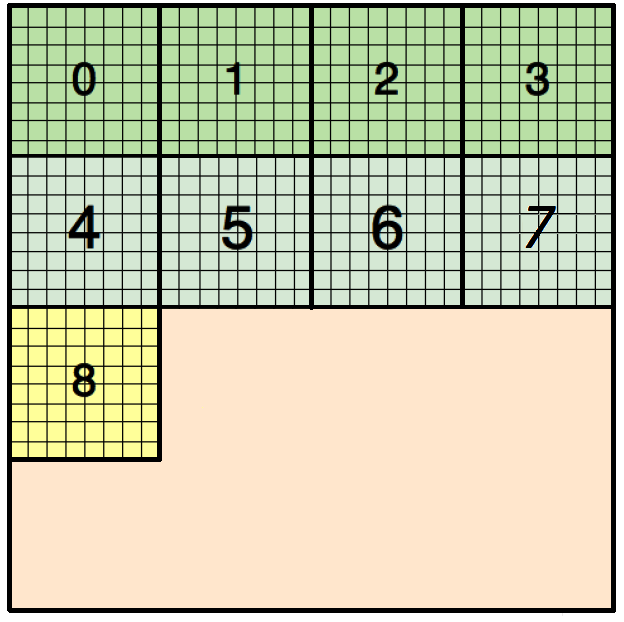
\includegraphics[width=0.3\textwidth]{Immagini/block_on_grid.png}
	\caption{Figura con singola immagine}
	\label{fig:one}
\end{figure}

\begin{figure}[ht]
	\centering
	\begin{subfigure}{0.3\textwidth}
		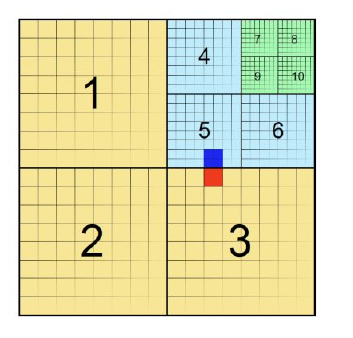
\includegraphics[width=1.0\textwidth]{Immagini/disoposizione_blocchi_fisica.png}
		\caption{Disposizione fisica dei blocchi}
	\end{subfigure}%
	\begin{subfigure}{0.3\textwidth}
		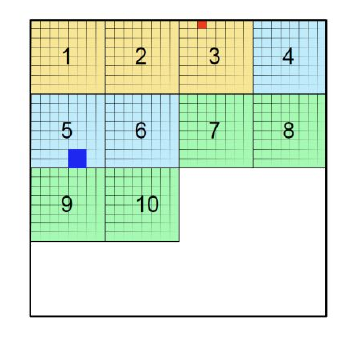
\includegraphics[width=1.0\textwidth]{Immagini/disoposizione_blocchi_logica.png}
		\caption{Disposizione logica dei blocchi}
	\end{subfigure}
	\caption{Figura con due immagini}
	\label{fig:two}
\end{figure}


\begin{figure}[H]
	\centering
	\begin{subfigure}{0.5\textwidth}
		\centering
		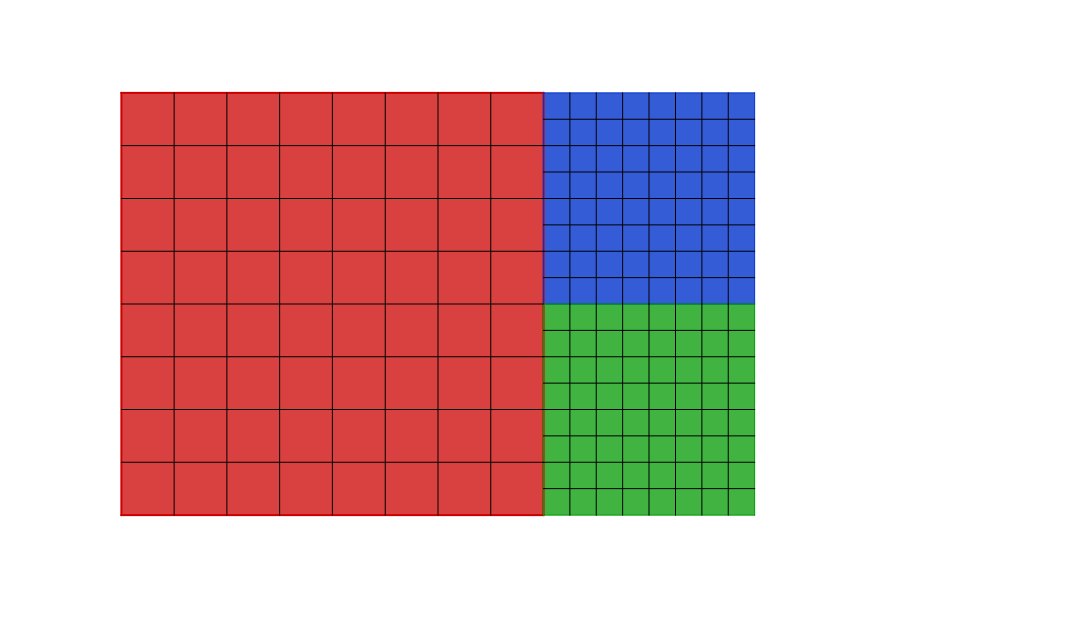
\includegraphics[width=0.7\linewidth]{Immagini/lev_less1.png}
		\caption{\textit{lev} = -1\newline}
		\label{fig:test1}
	\end{subfigure}%
	\begin{subfigure}{0.5\textwidth}
		\centering
		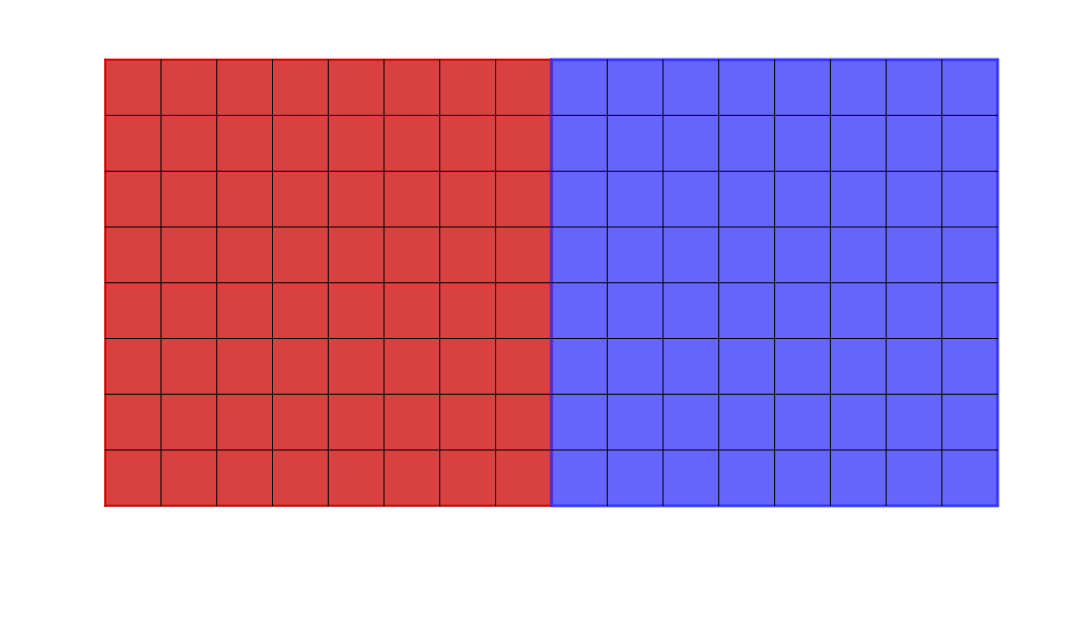
\includegraphics[width=0.7\linewidth]{Immagini/lev0.png}
		\caption{\textit{lev} = 0\newline}
		\label{fig:test2}
	\end{subfigure}
	\begin{subfigure}{0.7\textwidth}
		\centering
		\begin{subfigure}{0.5\textwidth}
			\centering
			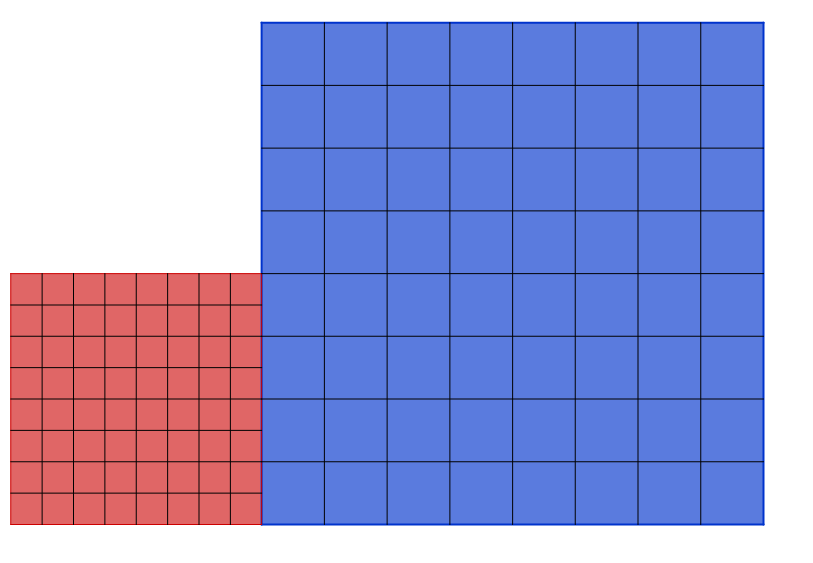
\includegraphics[width=0.5\linewidth]{Immagini/bloccomaggiore1.png}
		\end{subfigure}%
		\begin{subfigure}{0.5\textwidth}
			\centering
			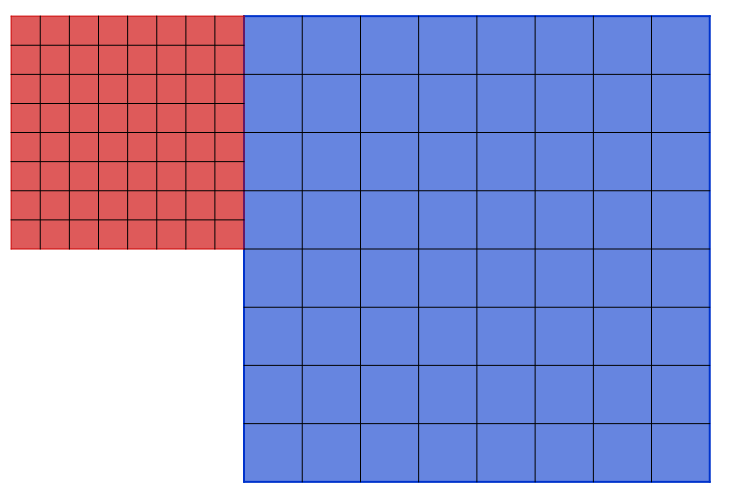
\includegraphics[width=0.5\linewidth]{Immagini/bloccomaggiore2.png}
		\end{subfigure}
		\caption{\textit{lev} = 1}
		\label{fig:lev1}
	\end{subfigure}
	\caption{Figura con tre immagini (di cui una composta da due sotto-immagini)}
	\label{fig:three}
\end{figure}

\section{Esempi di Codice e Misc.}\label{sec:code}
Alcuni esempi di codice, definizioni, tabelle e altro.

\begin{algorithm}[ht]
	\caption{Esempio di pseudo-codice}
	\label{alg:Prim_Mst}
	\begin{algorithmic}[1]
		\Statex
		\Function{MST-Prim}{grafo G, funzione\_peso $\omega$, nodo\_radice r}\\
		\State{\textit{Q}: coda di priorita contenente tutti i vertici in \textit{V}}
		\For{ogni \textit{u} $\in$ V(G)}
		\Let{\textit{u.key}}{$\infty$}
		\Let{\textit{u.}$\pi$}{\textit{NIL}} 
		\EndFor
		\Let{\textit{r.key}}{0}
		\Let{\textit{Q}}{\textit{V(G)}}
		\While{\textit{Q} $\neq$ 0}
		\Let{\textit{u}}{EXTRACT-MIN(\textit{Q})}
		\For{ogni \textit{v} $\in$ \textit{G.Adj[u]}}
		\If{$v \in Q$ and $\omega(u,v) < v.key$}
		\Let{\textit{v.key}}{$\omega(u,v)$}
		\Let{\textit{v.}$\pi$}{\textit{v}}
		\EndIf
		\EndFor
		\EndWhile
		\State \Return{}
		\EndFunction
	\end{algorithmic}
\end{algorithm}

\begin{minipage}{\textwidth}
\begin{lstlisting}[caption={Esempio di definizione struttura dati C++, ma non algoritmo},
	label={lst:block_struct}]
	struct Block
	{
		int id_block;
		char resolution;
		int id_subdomain;
		int key;
		bool in_other_subdomain;
		struct neigh_t neighbors[4];
	};
\end{lstlisting}
\end{minipage}



\begin{algorithm}[ht]
	\caption{Esempio di codice imperativo}
	\label{alg:my_prim_multi}
	\begin{algorithmic}[1]
		\Statex
		\Function{PRIM\_MULTI-MST}{roots\_list \textit{roots}, array\_Block \textit{adjacency\_list}}
		
		\State{\color{blue}{//Inizializzazione di tutti i vertici}}
		\For{ogni \textit{u} $\in$ \textit{adjacency\_list}}
		\Let{\textit{u.key}}{$\infty$}
		\Let{\textit{u.id\_subdomains}}{\textit{NIL}}
		\Let{\textit{u.in\_other\_subdomain}}{FALSE} 
		\EndFor
		
		\State{\color{blue}{//Inizializzazione di tutte le radici}}
		\Let{\textit{i}}{0}
		\For{ogni \textit{r} $\in$ \textit{roots}}
		\Let{\textit{r.key}}{0}
		\Let{\textit{r.id\_subdomains}}{\textit{i}}
		\Let{\textit{i}}{$i+1$}
		\EndFor
		\State{\textit{Q}: coda di priorita ordinata in base al campo 
			\textit{key}}
		\Let{\textit{Q}}{\textit{roots}}
		\Let{\textit{count}}{0}
		
		\While{count $<$ \textit{adjacency\_list.size}}
		\Let{\textit{u}}{EXTRACT-MIN(\textit{Q})}
		
		\If{!(\textit{u.in\_other\_subdomain})}
		\State{\color{blue}{//Essendo il minimo viene aggiunto definitivamente}}
		\Let{\textit{u.in\_other\_subdomain}}{TRUE}
		\State{\color{blue}{//Si analizzano i vicini}}
		\For{ogni \textit{v} $\in$ \textit{u.neighbors}}
		\State{\color{blue}{//In questo caso specifico il peso di ogni arco vale 1}}
		\If{$v \in adjacency\_list$ and ($u.key+1) < v.key$}
		\Let{\textit{v.key}}{$u.key+1$}
		\Let{\textit{v.subdomains}}{\textit{u.subdomains}}
		\Let{\textit{count}}{\textit{count} + 1}
		\EndIf
		\EndFor
		\EndIf
		\EndWhile
		\State \Return{}
		\EndFunction
	\end{algorithmic}
\end{algorithm}

\begin{algorithm}[ht]
	\caption{esempio di algoritmo in C++}
	\label{lst:genic_mpi}
	\begin{lstlisting}
		#include (*@\textquotedblleft@*)mpi.h"
		
		(*@~ ~ ~ ~\raisebox{-1pt}[0pt][0pt]{$\vdots$}@*)
		
		main(int argc, char** argv){
			
			(*@~ ~ ~ ~ ~ ~ ~ ~ ~ ~{\raisebox{-1pt}[0pt][0pt]{$\vdots$}}@*)
			
			//Nessuna chiamata a funzioni MPI prima di questa
			MPI_Init(&argc, &argv);
			
			(*@~ ~ ~ ~ ~ ~ ~ ~ ~ ~{\raisebox{-1pt}[0pt][0pt]{$\vdots$}}@*)
			
			MPI_Finalize();
			//Nessuna chiamata a funzioni MPI dopo questa
			
			(*@~ ~ ~ ~ ~ ~ ~ ~ ~ ~{\raisebox{-1pt}[0pt][0pt]{$\vdots$}}@*)
		}	
	\end{lstlisting}
\end{algorithm}

\begin{defn}[Esempio di Definizione]
	Un piccolo esempio di definizione
\end{defn}

\begin{table}[ht]
	\centering
	\resizebox{0.99\linewidth}{!}{
		\begin{tabular}{||c||c|c|c|c|c|c|c|c|c|c||}
			\hhline{|t:=:t:==========:t|}
			CT scan &\phantom{00}01\phantom{00}&\phantom{00}02\phantom{00}&\phantom{00}03\phantom{00}&\phantom{00}04\phantom{00}&\phantom{00}05&\phantom{00}06\phantom{00}&\phantom{00}07\phantom{00}&\phantom{00}08\phantom{00}&\phantom{00}09\phantom{00}&\phantom{00}10\phantom{00} \\
			\hhline{|:=::==========:|}
			Input arteries (n.) &66&175&76&134&198&172&154&108&91&65 \\
			\hhline{||-||----------||}
			Labeling time (s)&19.13&87.38&26.11&47.08&90.89&356.95&303.77&91.95&16.01&21.88 \\
			\hhline{||-||----------||}
			Grounding time (s)&9.76&52.45&9.57&22.88&70.34&47.52&37.44&17.98&10.61&8.04 \\
			\hhline{||-||----------||}
			Optimum time (s)&6.66&31.05&14.67&20.63&15.2&29.17&54.71&61.03&4.28&7.24 \\
			\hhline{|b:=:b:==========:b|}
		\end{tabular}
	}
	\vspace*{2mm}
	\caption{Esempio di tabella}
	\label{tab:perf}
\end{table}


\section{Citazioni}
Durante la scrittura della Tesi è necessario fornire i riferimenti bibliografici che hanno permesso la stesura della tesi stessa.
Questo si ottiene semplicemente tramite l'utilizzo del comando ``cite'' che prende come argomento la label di una delle entry nel file .bib.
Quindi per citare una qualunque fonte, ad esempio ``Artificial Intelligence - A Modern Approach", si può fare \cite{modernApproach} ($\backslash\text{cite}\{\text{modernApproach}\}$).
Questo leggerà la referenza nel file .bib che ha come label ``cormen".
Per citare più riferimenti contemporaneamente basta sperare le varie labels con una virgola come segue \cite{gelfond1998action,modernApproach,durfee1999distributed,de2003resource,allen2009complexity,bernstein2002complexity}.
Le reference non citate non appariranno in bibliografia.
\href{https://dblp.uni-trier.de/}{dblp} e \href{https://scholar.google.com/}{Google Scholar} sono siti nei quali estrarre la reference per bibtex per un lavoro di cui si conosce solo il titolo, ad esempio.
\chapter{Background}\label{chapter:background}
\section{Teoria degli insiemi}
\begin{definition}[Insieme]
Un \textit{insieme} è una collezione di elementi. Lo si può descrivere in due modi: 
\begin{itemize}
    \item estensionalmente: come elenco degli elementi presenti nell'insieme separati da virgole e contenuti tra parentesi graffe;
    \item per proprietà caratteristica: come l'insieme di oggetti che soddisfano una proprietà P, con questa sintassi \(\{x\ |\ \textrm{P}(x)\}\);
\end{itemize}
\end{definition}

\begin{definition}[Appartenenza]
Se un elemento \(x\) fa parte di un insieme \(X\) diremo che \(x\) \textit{appartiene} ad \(X\) e scriviamo \(x\in X\), altrimenti \(x \notin X\).
\end{definition}

\begin{definition}[Cardinalità]
La \textit{cardinalità} di un insieme \(X\) è il numero di elementi al suo interno e lo si denota con \(|X|\). Un insieme può avere un numero infinito di elementi. Un insieme con cardinalità 0 è detto \textit{insieme vuoto} e viene rappresentato con \(\{\}\) oppure \(\emptyset\).
\end{definition}

\begin{definition}[Operazioni sugli insiemi]
Esistono numerose operazioni applicabili agli insiemi, le principali sono:
\begin{itemize}
    \item \textit{unione}: l'unione di due insiemi \(A, B\) si scrive \(A\cup B\) e deonota l'insieme contenente tutti gli elementi di \(A\) o di \(B\) o di entrambi;
    \item \textit{intersezione}: l'intersezione di due insiemi \(A, B\) si scrive \(A\cap B\) e deonota l'insieme contenente tutti gli elementi presenti sia in \(A\) che in \(B\);
    \item \textit{differenza}: la differenza tra un insieme \(A\) ed un insieme \(B\) si scrive \(A\setminus B\) e deonota l'insieme contenente tutti gli elementi di \(A\) non presenti in \(B\);
\end{itemize}
\end{definition}

\begin{definition}[Relazioni tra insiemi]
Due insiemi \(A, B\) si dicono:
\begin{itemize}
    \item \textit{congiunti} se sono lo stesso insieme, ovvero se \(A\setminus B=B\setminus A=\emptyset\);
    \item \textit{disgiunti}  se non hanno elementi in comune, ovvero \(A\cap B=\emptyset\);
\end{itemize}
Si dice che \(B\) è \textit{sottoinsieme} di \(A\) se \(A\) contiene tutti gli elementi di \(B\) e si scrive \(B\subseteq A\). Se vogliamo escludere che \(B\) coincida con \(A\) scriviamo \(B\subset A\). 
\end{definition}

\begin{definition}[Insieme delle parti]
Dato un qualisasi insieme \(A\) si definisce \textit{insieme delle parti} l'insieme che contiene tutti e soli i sottoinsiemi di \(A\), lo denotiamo con \(\wp(A)=\{B\ |\ B\subseteq A\}\).
\end{definition}

\begin{definition}[Prodotto cartesiano]
Il \textit{prodotto cartesiano} degli insiemi \(X_1,X_2,\cdots,X_n\) è l'insieme di tutte le n-uple dove il primo elemento appartiene a \(X_1\), il secondo a \(X_2\) e così via. Formalmente si scrive \(X_1\times X_2\times\cdots\times X_n=\{\langle x_1, x_2,\cdots, x_n\rangle\ |\ x_1\in X_1\wedge x_2\in X_2\wedge\cdots\wedge x_n\in X_n\}\)
\end{definition}

\begin{definition}[Relazione]
Una \textit{relazione} R tra gli insiemi \(X_1,X_2,\cdots,X_n\) è un sottoinsieme del prodotto cartesiano \(X_1\times X_2\times\cdots\times X_n\). Gli elementi \(x_i\) con \(i\in [\, n]\) sono in relazione R se \(\langle x_1, x_2,\cdots, x_n\rangle\in\textrm{R}\). Un relazione \(\textrm{R}_b\) definita tra due insiemi \(X, Y\) si dice relazione binaria, se due elementi \(x, y\) sono in relazione \(\textrm{R}_b\) tra di loro scriveremo \(x\textrm{R}_b y\).
\end{definition}

\begin{definition}[Relazione di ordine parziale]
Una relazione binaria \(\preceq\) sull'insieme \(S\) è una \textit{relazione di ordine parziale} se possiede queste tre proprietà:
\begin{itemize}
\item Riflessività: \(\forall s\in S. s\preceq s\);
\item Antisimmetrica: \(\forall s_1, s_2\in S. s_1\preceq s_2 \wedge s_2\preceq s_1 \Rightarrow s_1=s_2\);
\item Transitività: \(\forall s_1, s_2, s_3 \in S. s_1\preceq s_2 \wedge s_2\preceq s_3 \Rightarrow s_1\preceq s_3\);
\end{itemize}
\end{definition}

\section{Teoria degli ordini}
\begin{definition}[Insieme parzialmente ordinato]
Un \textit{insieme parzialmente ordinato} (o poset) è una coppia \(\langle S, \preceq\rangle\) dove \(S\) è un insieme di elementi e \(\preceq\) è una relazione di ordine parziale su \(S\).
\end{definition}

\begin{definition}[Catena]
Una catena di un poset \(\simplePoset{S}\) è un sottoinsieme \(C\subseteq S\) tale che: \(\forall c_1, c_2 \in C. c_1\preceq_{S} c_2 \vee c_2\preceq_{S} c_1\)
\end{definition}

\begin{definition}[Copertura]
Dato un poset \(\simplePoset{S}\) e due elementi \(s_1, s_2 \in S\) diciamo che \(s_1\) \textit{copre} \(s_2\) se non esiste un altro elemento \(s_3\in S\) tale che \(s_1 \preceq_{S} s_3 \preceq_{S} s_2\).
\end{definition}

\begin{definition}[Diagramma di Hasse]
\'E possibile visualizzare un insieme parzialmente ordinato \(\simplePoset{S}\) attraverso un \textit{diagramma di Hasse}. Un diagramma di Hasse è un grafo i cui nodi sono gli elementi dell'isnsieme \(S\) del poset e un arco viene disegnato tra due elementi \(s_1, s_2 \in S\) solo se \(s_1\) copre \(s_2\).
\end{definition}

\begin{example} 
Se prendiamo l'insieme \(\textrm{Sign}=\{\perp, +, -, 0, 0+, 0-, \top\}\) e l'ordinamento parziale \(\preceq_{\textrm{Sign}}\) definito dal diagramma di Hasse in figura \ref{fig:signDomain} allora \(\simplePoset{\textrm{Sign}}\) è un insieme parzialmente ordinato.

\begin{figure}
\begin{center}
\begin{scriptsize}
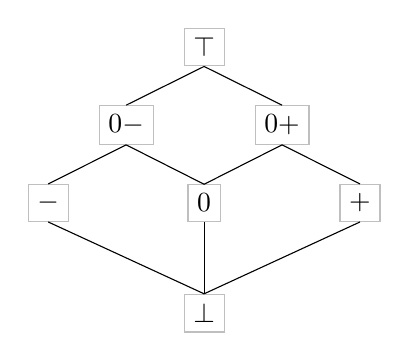
\begin{tikzpicture}
[align=center,node distance=1.4cm]
\node [rectangle,draw=black!25] (top) {\(\top\)};
\node [rectangle,draw=black!25] (zeroplus) [below right of=top]{\(0+\)};
\node [rectangle,draw=black!25] (zerominus) [below left of=top]{\(0-\)};
\node [rectangle,draw=black!25] (zero) [below left of=zeroplus]{\(0\)};
\node [rectangle,draw=black!25] (plus) [below right of=zeroplus]{\(+\)};
\node [rectangle,draw=black!25] (minus) [below left of=zerominus]{\(-\)};
\node [rectangle,draw=black!25] (bottom) [below of=zero]{\(\perp\)};

\draw (top.270) -- (zeroplus.90);
\draw (top.270) -- (zerominus.90);
\draw (zerominus.270) -- (minus.90);
\draw (zeroplus.270) -- (plus.90);
\draw (zerominus.270) -- (zero.90);
\draw (zeroplus.270) -- (zero.90);
\draw (bottom.90) -- (plus.270);
\draw (bottom.90) -- (zero);
\draw (bottom.90) -- (minus.270);
\end{tikzpicture}
\end{scriptsize}
\end{center}
\caption{diagramma di Hasse del dominio dei segni.}
\label{fig:signDomain}
\end{figure}
\end{example}

\begin{definition}[Condizione di catena ascendnente]
Un poset \(\simplePoset{S}\) soddisfa la \textit{condizione di catena ascendnente} (ACC) se e solo se ogni sequenza infinita \(\emph{s}_0\preceq\emph{s}_1\preceq\cdots\preceq\emph{s}_k\preceq\cdots\) di elementi di \emph{S} se: \(\exists\emph{n}\in\mathbb{N}.\ \emph{s}_m=\emph{s}_n\forall\emph{m}\geq\emph{n}\).
\end{definition}

\begin{definition}[Condizione di catena discendnente]
Un poset \(\simplePoset{S}\) soddisfa la \textit{condizione di catena discendnente} (DCC) se e solo se ogni sequenza infinita \(\emph{s}_0\succeq\emph{s}_1\succeq\cdots\succeq\emph{s}_k\succeq\cdots\) di elementi di \emph{S} se: \(\exists\emph{n}\in\mathbb{N}.\ \emph{s}_m=\emph{s}_n\forall\emph{m}\geq\emph{n}\).
\end{definition}

\begin{definition}[Upper bound e lub]
Dato un poset \(\simplePoset{S}\) e \(X\subseteq S\), \emph{l} è l'\textit{upper bound} di \emph{X} se \(\forall x\in X. x\preceq l\). Se l'insieme degli upper bound di \emph{X} ha un minimo questo lo chiamiamo \textit{least upper bound} (lub) e lo si denota con \(\bigsqcup X\). Se abbiamo l'insieme \(X=\{x_1, x_2\}\) (cioè composto da due elementi) possiamo scrivere equivalentemente \(\bigsqcup X=x_1\sqcup x_2\).
\end{definition}

\begin{definition}[Lower bound e glb]
Dato un poset \(\simplePoset{S}\) e \(X\subseteq S\), \emph{g} è il \textit{lower bound} di \emph{X} se \(\forall x\in X. x\succeq g\). Se l'insieme dei lower bound di \emph{X} ha un massimo questo lo chiamiamo \textit{greatest lower bound} (glb) e lo si denota con \(\bigsqcap X\). Se abbiamo l'insieme \(X=\{x_1, x_2\}\) (cioè composto da due elementi) possiamo scrivere equivalentemente \(\bigsqcap X=x_1\sqcap x_2\).
\end{definition}

\begin{definition}[Insieme parzialmente ordinato completo]
Un poset \(\simplePoset{S}\) è \textit{completo} se ogni catena crescente \(C\subseteq S\) ha un least upper-bound in \(S\), ovvero \(\bigsqcup C \in S\).
\end{definition}

\begin{definition}[Top e bottom] 
Un elemento \(\emph{x}\in\emph{S}\) di un poset \(\simplePoset{S}\) è l'elemento \textit{top} \(\top\) se \(\forall\emph{y}\in\emph{S}.\emph{y}\preceq\emph{x}\). Mentre è l'elemento \textit{bottom} \(\perp\) se \(\forall\emph{y}\in\emph{S}.\emph{x}\preceq\emph{y}\).
\end{definition}

\begin{definition}[Join semi reticolo]
Un \textit{join semi reticolo} \(\langle S,\preceq_S, \sqcup\rangle\) è un poset \(\simplePoset{S}\) tale che \(\forall x, y\in S\) esiste il lub \(x\sqcup y\).
\end{definition}

\begin{definition}[Meet semi reticolo]
Un \textit{meet semi reticolo} \(\langle\emph{S },\preceq_S, \sqcap\rangle\) è un poset \(\simplePoset{S}\) tale che \(\forall x, y\in S\) esiste il glb \(x\sqcap y\).
\end{definition}

\begin{definition}[Reticolo]
Un \textit{reticolo} \(\simpleLattice{S}\) è sia un join semi reticolo che un meet semi reticolo.
\end{definition}

\begin{definition}[Reticolo completo]
Un reticolo \(\simpleLattice{S}\) è un \textit{reticolo completo} se: \(\forall D\subseteq S.\bigsqcup D,\bigsqcap D\in S\). Una conseguenza di ciò è che esistono gli elementi top e bottom. Per questo possiamo scrivere un reticolo completo come \(\completeLattice{S}\).
\end{definition}

\begin{example}
Dato un insieme \(A\) non vuoto qualsiasi \(\langle\wp(A), \subseteq, \cup, \cap, A, \emptyset\rangle\) è un reticolo completo.
\end{example}

\begin{example}
Mostriamo un'altro esempio di reticolo completo. Il dominio del reticolo è l'insieme:
\[\textrm{Int}=\{[l, u]\ |\ l, u\in\mathbb{Z} \wedge l\leq u\} \cup \{[-\infty, u]\ |\ u\in\mathbb{Z}\} \cup \{[l, +\infty]\ |\ l\in\mathbb{Z}\} \cup \{\perp, \top\}\]
l'elemento \(\top\) equivale a \([-\infty, +\infty]\) e l'elemento \(\perp\) all'insieme vuoto [ ].
La relazione di ordine parziale \(\preceq\) è così definita: per ogni \([l_1, u_1], [l_2, u_2]\in\textrm{Int}\) si ha che \([l_1, u_1]\preceq_{\textrm{Int}} [l_2, u_2]\) se e solo se \(l_2\leq l_1 \wedge u_1\leq u_2\). Infine definiamo un operatore di lub \(\sqcup\) e di glb \(\sqcap\) così: per ogni \([l_1, u_1], [l_2, u_2]\in\textrm{Int}\) si ha che 
\begin{itemize}
\item \([l_1, u_1]\sqcup [l_2, u_2] = [\textrm{min}(l_1, l_2), \textrm{max}(u_1, u_2)]\)
\item \([l_1, u_1]\sqcap [l_2, u_2] = \) 
	$
	\begin{cases}
	[l_1, u_1] & \textrm{se } [l_1, u_1]\preceq [l_2, u_2] \\
	[l_2, u_2] & \textrm{se } [l_2, u_2]\preceq [l_1, u_1] \\
	\perp      & \textrm{se } (u_1 < l_2 \wedge l_1 < l_2) \vee (u_2 < l_1 \wedge l_2 < l_1) \\
	[l_2, u_1] & \textrm{se } l_1<l_2\leq u_1 \wedge l_2\leq u_1<u_2 \\
	[l_1, u_2] & \textrm{se } l_2<l_1\leq u_2 \wedge l_1\leq u_1<u_1
	\end{cases} 
	$
 
    questo significa semplicemente che dobbiamo prendere l'intersezione dei due intervalli e se l'intersezione è nulla restituiamo \(\perp\).
\end{itemize}
Abbiamo quindi un reticolo completo \(\langle\textrm{Int}, \preceq_{\textrm{Int}}, \sqcup, \sqcap, [-\infty, +\infty], [\ ] \rangle\). In oltre è possibile visualizzare l'ordinamento parziale sull'insieme Int attraverso il diagramma di Hasse (ovviamente incompleto) in figura \ref{fig:intervalDomain} :

\begin{figure}
\begin{center}
\begin{scriptsize}
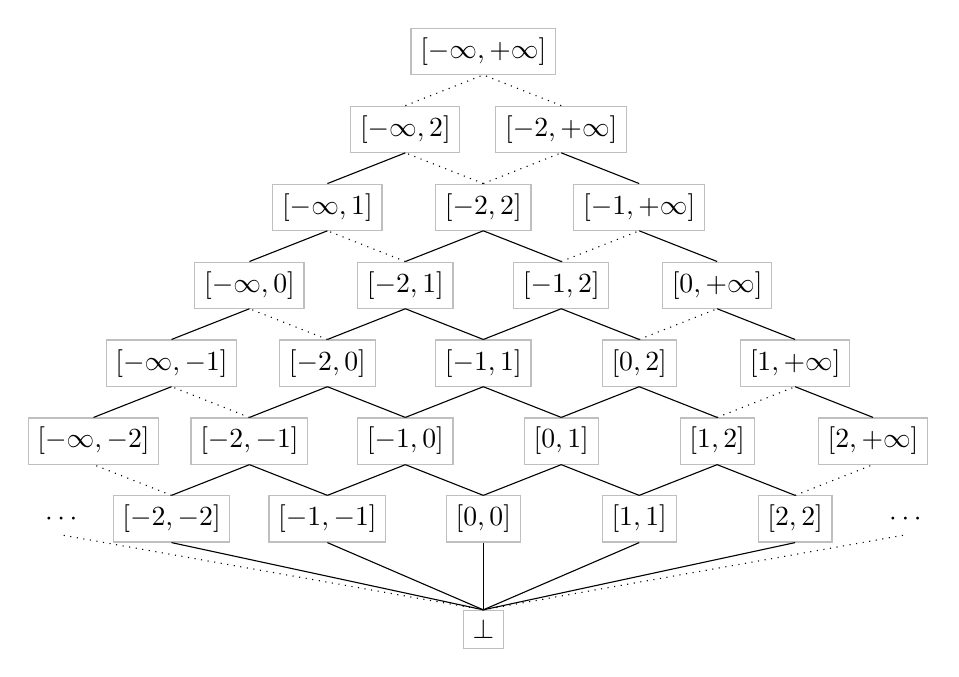
\begin{tikzpicture}
[align=center,node distance=1.4cm]
\node [rectangle,draw=black!25] (top) {\([-\infty, +\infty]\)};

\node [rectangle,draw=black!25] (minusInfto2) [below left of=top] {\([-\infty, 2]\)};
\node [rectangle,draw=black!25] (minusInfto1) [below left of=minusInfto2] {\([-\infty, 1]\)};
\node [rectangle,draw=black!25] (minusInftozero) [below left of=minusInfto1] {\([-\infty, 0]\)};
\node [rectangle,draw=black!25] (minusInftominus1) [below left of=minusInftozero] {\([-\infty, -1]\)};
\node [rectangle,draw=black!25] (minusInftominus2) [below left of=minusInftominus1] {\([-\infty, -2]\)};

\node [rectangle,draw=black!25] (minus2toInf) [below right of=top] {\([-2, +\infty]\)};
\node [rectangle,draw=black!25] (minus1toInf) [below right of=minus2toInf] {\([-1, +\infty]\)};
\node [rectangle,draw=black!25] (zerotoInf) [below right of=minus1toInf] {\([0, +\infty]\)};
\node [rectangle,draw=black!25] (plus1toInf) [below right of=zerotoInf] {\([1, +\infty]\)};
\node [rectangle,draw=black!25] (plus2toInf) [below right of=plus1toInf] {\([2, +\infty]\)};

\node [rectangle,draw=black!25] (minus2to2) [below left of=minus2toInf] {\([-2, 2]\)};
\node [rectangle,draw=black!25] (minus2to1) [below left of=minus2to2] {\([-2, 1]\)};
\node [rectangle,draw=black!25] (minus1to2) [below right of=minus2to2] {\([-1, 2]\)};

\node [rectangle,draw=black!25] (minus1to1) [below right of=minus2to1] {\([-1, 1]\)};
\node [rectangle,draw=black!25] (minus2tozero) [below left of=minus2to1] {\([-2, 0]\)};
\node [rectangle,draw=black!25] (zeroto2) [below right of=minus1to2] {\([0, 2]\)};

\node [rectangle,draw=black!25] (zeroto1) [below right of=minus1to1] {\([0, 1]\)};
\node [rectangle,draw=black!25] (minus1tozero) [below left of=minus1to1] {\([-1, 0]\)};
\node [rectangle,draw=black!25] (plus1to2) [below right of=zeroto2] {\([1, 2]\)};
\node [rectangle,draw=black!25] (minus2tominus1) [below left of=minus2tozero] {\([-2, -1]\)};

\node [rectangle,draw=black!25] (minus2) [below left of=minus2tominus1] {\([-2, -2]\)};
\node [rectangle,draw=black!25](minus1) [below left of=minus1tozero] {\([-1, -1]\)};
\node [rectangle,draw=black!25](zero) [below left of=zeroto1] {\([0, 0]\)};
\node [rectangle,draw=black!25] (plus1) [below left of=plus1to2] {\([1, 1]\)};
\node [rectangle,draw=black!25] (plus2) [below right of=plus1to2] {\([2, 2]\)};

\node [rectangle,draw=black!25] (bottom) [below of=zero] {\(\perp\)};

\node (minusdots) [left of=minus2] {\(\cdots\)};
\node (plusdots) [right of=plus2] {\(\cdots\)};


\draw (bottom.90) -- (zero.270);
\draw (bottom.90) -- (plus1.270);
\draw (bottom.90) -- (plus2.270);
\draw (bottom.90) -- (minus2.270);
\draw (bottom.90) -- (minus1.270);
\draw[dotted] (bottom.90) -- (plusdots.270);
\draw[dotted] (bottom.90) -- (minusdots.270);

\draw (zero.90) -- (minus1tozero.270);
\draw (zero.90) -- (zeroto1.270);
\draw (plus1.90) -- (plus1to2.270);
\draw (plus1.90) -- (zeroto1.270);
\draw (minus1.90) -- (minus1tozero.270);
\draw (minus1.90) -- (minus2tominus1.270);
\draw (minus2.90) -- (minus2tominus1.270);
\draw (plus2.90) -- (plus1to2.270);

\draw (minus2tominus1.90) -- (minus2tozero.270);
\draw (minus1tozero.90) -- (minus2tozero.270);
\draw (minus1tozero.90) -- (minus1to1.270);
\draw (zeroto1.90) -- (minus1to1.270);
\draw (zeroto1.90) -- (zeroto2.270);
\draw (plus1to2.90) -- (zeroto2.270);

\draw (minus1to1.90) -- (minus2to1.270);
\draw (minus1to1.90) -- (minus1to2.270);
\draw (minus2tozero.90) -- (minus2to1.270);
\draw (zeroto2.90) -- (minus1to2.270);

\draw (minus2to1.90) -- (minus2to2.270);
\draw (minus1to2.90) -- (minus2to2.270);

\draw (minusInftominus2.90) -- (minusInftominus1.270);
\draw (minusInftominus1.90) -- (minusInftozero.270);
\draw (minusInftozero.90) -- (minusInfto1.270);
\draw (minusInfto1.90) -- (minusInfto2.270);

\draw (plus2toInf.90) -- (plus1toInf.270);
\draw (plus1toInf.90) -- (zerotoInf.270);
\draw (zerotoInf.90) -- (minus1toInf.270);
\draw (minus1toInf.90) -- (minus2toInf.270);

\draw[dotted] (minus2.90) -- (minusInftominus2.270);
\draw[dotted] (minus2tominus1.90) -- (minusInftominus1.270);
\draw[dotted] (minus2tozero.90) -- (minusInftozero.270);
\draw[dotted] (minus2to1.90) -- (minusInfto1.270);
\draw[dotted] (minus2to2.90) -- (minusInfto2.270);

\draw[dotted] (plus2.90) -- (plus2toInf.270);
\draw[dotted] (plus1to2.90) -- (plus1toInf.270);
\draw[dotted] (zeroto2.90) -- (zerotoInf.270);
\draw[dotted] (minus1to2.90) -- (minus1toInf.270);
\draw[dotted] (minus2to2.90) -- (minus2toInf.270);

\draw[dotted] (minusInfto2.90) -- (top.270);
\draw[dotted] (minus2toInf.90) -- (top.270);

\end{tikzpicture}
\end{scriptsize}
\end{center}
\caption{rappresentazione incompleta del diagramma Hasse del dominio degli intervalli interi}
\label{fig:intervalDomain}
\end{figure}

Si può osservare come questo ordinamento non rispetta ne la condizione di catena ascendente ne la condizione di catena discendente.
\end{example}

\begin{definition}[Funzione parziale]
Una \textit{funzione parziale} \(f\) da \(A\) a \(B\), denotata \(f:A\rightharpoonup B\), è un sottoinsieme del prodotto cartesiano \(A\times B\) che associa ogni un elemento di \(A\) ad al massimo un elemento di \(B\). Scriviamo \(f(x)=y\) se la coppia \(\langle x, y\rangle\in f\). Definiamo il \textit{dominio} di una funzione parziale \(f:A\rightharpoonup B\) così: \(\textrm{dom}(f)=\{x\in A\ |\ \exists y\in B:f(x)=y\}\). L'insieme di tutte le funzioni parziali da \(A\) a \(B\) si scrive \(A\rightharpoonup B\).
\end{definition}

\begin{definition}[Funzione totale]
Una \textit{funzione totale} \(f\) da \(A\) a \(B\), denotata \(f:A\rightarrow B\), è una funzione parziale che associa ad ogni elemento di \(A\) esattamente un elemento di \(B\). Ovvero \(\textrm{dom}(f)=A\). L'insieme di tutte le funzioni totali si scrive \(A\rightarrow B\).
\end{definition}

\begin{definition}[Proprietà di una funzione]
Una funzione \(f:A\rightarrow B\) può essere:
\begin{itemize}
    \item \textit{suriettiva} se \(\forall y\in B : \exists x\in A: f(x)=y\);
    \item \textit{iniettiva} se \(\forall x,y\in A : f(x)=f(y)\Rightarrow x=y\);
    \item \textit{biiettiva} se è sia suriettiva che iniettiva;
\end{itemize}
Dati due poset \(\simplePoset{A}\) e \(\simplePoset{B}\) una funzione \(f:A\rightarrow B\) è detta:
\begin{itemize}
    \item \textit{monotona} se \(\forall x,y\in A, x\preceq_A y\Rightarrow f(x)\preceq_B f(y)\);
    \item \textit{continua} (o \textit{Scott-continua}) se per ogni catena \(C\subseteq A\), se \(\bigsqcup C\) esiste allora \(f(\bigsqcup C)=\bigsqcup\{f(x)\ |\ x\in C\}\);
    \item \textit{cocontinua} (o \textit{Scott-cocontinua}) se per ogni catena \(C\subseteq A\), se \(\bigsqcap C\) esiste allora \(f(\bigsqcap C)=\bigsqcap\{f(x)\ |\ x\in C\}\);
\end{itemize}
\end{definition}

\section{Teoria del fix-point}

\begin{definition}[Fix-point, pre-fix-point, post-fix-point]
Dato un \(\simplePoset{S}\) ed una funzione \(f:S\rightarrow S\) possiamo definire:
\begin{itemize}
\setlength\itemsep{0em}
	\item i fixpoint di \emph{f} quegli elementi \(s\in S\) tali che \(f(s)=s\), denotati con \(\textrm{fp}(f)\).
	\item i pre-fixpoint di \emph{f} quegli elementi \(s\in S\) tali che \(s\preceq_S f(s)\), denotati con \(\textrm{prefp}(f)\).
	\item i post-fixpoint di \emph{f} quegli elementi \(s\in S\) tali che \(f(s)\preceq_S s\), denotati con \(\textrm{postfp}(f)\).
\end{itemize}
\end{definition}

\begin{definition}[least fix-point, greatest fix-point]
Dato un \(\simplePoset{S}\) ed una funzione \(f:S\rightarrow S\) il \textit{least fix-point} di \textit{f}, scritto \(\textrm{lfp}(f)\), è un fix-point di \textit{f} tale che \(\forall x\in\textrm{fp}(f):\textrm{lfp}(f)\preceq_S x\). Dualmente il \textit{greatest fix-point} di \textit{f}, \(\textrm{gfp}(f)\), è un fix-point di \textit{f} tale che \(\forall x\in\textrm{fp}(f):x\preceq_S \textrm{gfp}(f)\).
\end{definition}

\begin{theorem}[Teorema del fix-point di Tarski]
Dato un reticolo completo \(\completeLattice{S}\) ed una funzione monotona \(f:S\rightarrow S\), anche l'insieme dei fix-point di f è un reticolo completo. 
\end{theorem}

Questo teorema garantisce l'esistenza di fix-point, e più in particolare garantisce l'esistenza di un least fix-point, \(\textrm{lfp}(f)=\bigsqcap\textrm{postfp}(f)\), e di un greatest fix-point, \(\textrm{gfp}(f)=\bigsqcup\textrm{prefp}(f)\). Il teorema non da però un metodo costruttivo per ottenere tali fix-point, per questo motivo c'è il teorema seguente.

\begin{theorem}[Teorema del fix-point di Kleene]
Dato un insieme parzialmente ordinato completo \(\simplePoset{S}\) ed una funzione Scott-continua \(f:S\rightarrow S\) allora f ha un least fix-point ed è il least upper bound della seguente catena crescente:
\[\perp\preceq_S f(\perp) \preceq_S f(f(\perp)) \preceq_S f(f(f(\perp))) \preceq_S \cdots\]
ovvero \(\textrm{lfp}(f)=\bigsqcup\{f^n(\perp)\ |\ n\geq 0\}\).
\end{theorem}

Più generalmente si può partire da qualsiasi pre-fix-point \(s\in S\) di \(f\) ottenendo \(\textrm{lfp}_s(f)=\bigsqcup\{f^n(s)\ |\ n\geq 0\}\) che è il più piccolo fix-point maggiore o uguale di \(s\).

\section{Connessione di Galois}

\begin{definition}[Connessione di Galois]
Dati due poset \(\simplePoset{A}\) e \(\simplePoset{C}\) e due funzioni \(\alpha:C\rightarrow A\) e \(\gamma:A\rightarrow C\), la quadrupla \(\langle \simplePoset{C}, \alpha, \gamma, \simplePoset{A}\rangle\) è una connessione di Galois (in corto dall'inglese GC) se e solo se:
\[\forall a\in A, \forall c\in C: \alpha(c)\preceq_A a \Leftrightarrow c\preceq_C \gamma(a)\]
Una GC \(\langle \simplePoset{C}, \alpha, \gamma, \simplePoset{A}\rangle\) si denota \(\simplePoset{C}\galois{\alpha}{\gamma}\simplePoset{A}\).
\end{definition}

Data una connessione di Galois \(\simplePoset{C}\galois{\alpha}{\gamma}\simplePoset{A}\) le funzioni \(\alpha\) e \(\gamma\) si determinano univocamente a vicenda in questo modo:
\[\alpha(c) = \bigsqcap_A\{a\ |\ c\preceq_C \gamma(a)\}\]
\[\gamma(a) = \bigsqcup_C\{c\ |\ \alpha(c)\preceq_A a\}\]

Un'altra importante proprietà delle connessioni di Galois è che date due connessioni di Galois \(\simplePoset{C}\galois{\alpha_1}{\gamma_1}\simplePoset{A}\) e \(\simplePoset{A}\galois{\alpha_2}{\gamma_2}\simplePoset{B}\), la loro composizione \(\simplePoset{C}\galois{\alpha_1\circ\alpha_2}{\gamma_1\circ\gamma_2}\simplePoset{B}\) è anche una connessione di Galois.

\begin{example}\label{ex:galoisSignInt}
Prendiamo i due poset mostrati negli esempi di prima, \(\simplePoset{\textrm{Int}}\) e \(\simplePoset{\textrm{Sign}}\), diamo una definizione delle funzioni \(\alpha:\textrm{Int}\rightarrow\textrm{Sign}\) e \(\gamma:\textrm{Sign}\rightarrow\textrm{Int}\) tali da creare la connessione di Galois \(\GaloisConnection{\textrm{Int}}{\textrm{Sign}}\):
\begin{itemize}
\item dato \(i\in\textrm{Int}\) abbiamo che \(\alpha(i)\) = 
$
\begin{cases}
\perp_{\textrm{Sign}}  & \textrm{se } i=\perp_{\textrm{Int}}\\
0  & \textrm{se } i=[0, 0]\\
+  & \textrm{se } i=[l, u], \textrm{con } l, u \in\mathbb{Z}^+\\
-  & \textrm{se } i=[l, u], \textrm{con } l, u \in\mathbb{Z}^-\\
0+  & \textrm{se } i=[0, u], \textrm{con } u \in\mathbb{Z}^+\\
0-  & \textrm{se } i=[l, 0], \textrm{con } l \in\mathbb{Z}^-\\
\top_{\textrm{Sign}}  & \textrm{se } i=[l, u], \textrm{con } l\in\mathbb{Z}^- \textrm{e } u \in\mathbb{Z}^+\\
\end{cases}
$
\item dato \(s\in\textrm{Sign}\) abbiamo che \(\gamma(s)\) =
$
\begin{cases}
\perp_{\textrm{Int}}  & \textrm{se } s=\perp_{\textrm{Sign}}\\
[0, 0] & \textrm{se } s=0 \\
[1, +\infty] & \textrm{se } s=+\\
[-\infty, -1] & \textrm{se } s=-\\
[0, +\infty] & \textrm{se } s=0+\\
[-\infty, 0] & \textrm{se } s=0-\\
[-\infty, +\infty] & \textrm{se } s=\top_{\textrm{Sign}}\\
\end{cases}
$

\end{itemize}
\end{example}

\begin{example}
Anche i poset \(\simplePoset{\textrm{Int}}\) e \(\langle\wp(\mathbb{Z}), \subseteq\rangle\) formano una connessione di Galois se definiamo \(\alpha:\wp(\mathbb{Z})\rightarrow\textrm{Int}\) e \(\gamma:\textrm{Int}\rightarrow\wp(\mathbb{Z})\) in questo modo:
\begin{itemize}
\item dato \(p\in\wp(\mathbb{Z})\) si ha che \(\alpha(p)\) = 
$
\begin{cases}
\perp_{\textrm{Int}} & \textrm{se } p=\emptyset\\
[\textrm{min}(p), \textrm{max}(p)] & \textrm{altrimenti}\\
\end{cases}
$
    \item dato \(i=[l, u]\in\textrm{Int}\) si ha che \(\gamma(i)=\{z\ |\ l\leq z \leq u\}\);
\end{itemize}
dove le funzioni \(\textrm{min},\textrm{max}:\wp(\mathbb{Z})\rightarrow\mathbb{Z}\cup\{-\infty, +\infty\}\) possono restituire anche più/meno infinito nel caso l'insieme non sia vuoto ma non abbia un massimo/minimo (quindi se cresce/decresce all'infinito).
\end{example}

\section{Analisi statica ed Interpretazione astratta}

Lo scopo dell'\textit{analisi statica} è quello di provare formalmente certe proprietà di un programma. Per essere definita statica una analisi deve avere la caratteristica di non eseguire il codice (in caso opposto l'analisi si dice \textit{dinamica}, un esempio è il tradizionale metodo di debug con test), o meglio di non eseguirlo nella sua forma concreta. L'\textit{interpretazione astratta} è un modello matematico che può essere utilizzato per compiere analisi statica. L'idea basilare è quella di astrarre la computazione su un dominio astratto e interpretare il codice muovendoci in uno spazio di oggetti astratti che approssimano il dominio concreto. Per fare ciò dobbiamo creare una semantica astratta, che ragiona nel mondo del dominio astratto, che sia \textit{sound} in rispetto alla semantica concreta, la quale invece ragiona su un dominio concreto. Il motivo per cui ci accontentiamo di una approssimazione è che spesso lavorare sul dominio concreto risulta impossibile a causa dei limiti della computazione o è estremamente costoso in termini di tempo. Ci basta perciò una soluzione approssimata, ma corretta, da cui si spera sia possibile verificare certe proprietà del programma analizzato.

\subsection{Interpretazione astratta}
Un linguaggio \(\mathbb{L}\) mette a disposizione una semantica, ovvero una descrizione formale e matematica del comportamento di un programma \(\rho\) scritto in \(\mathbb{L}\) partendo da uno stato iniziale (che può rappresentare la collezione di elementi di input di \(\rho\)). Da tale semantica si possono ottenere diverse \textit{semantiche concrete}, ovvero funzioni \(\textbf{S}:Program_\mathbb{L}\rightarrow \mathbb{C}\),  che prendono un programma \(\rho\) in \(\mathbb{L}\) e restituiscono un oggetto dell'insieme \(\mathbb{C}\), detto \textit{dominio semantico concreto}, che ci dice qualcosa sul comportamento di \(\rho\) e attraverso cui è pssibile verificarne crete proprietà. Una caratteristica necessaria di un dominio concreto è che deve essere parte di un reticolo completo, per semplicità scriveremo \(\simplePoset{\mathbb{C}}\). Due esempi di semantiche concrete sono:
\begin{itemize}
    \item \textit{trace semantics}: il dominio concreto \(\mathbb{C}\) di questa semantica è l'insieme delle parti di tutte le tracce di esecuzione possibili (anche quelle infinite) per ogni possibile programma scritto in \(\mathbb{L}\) per ogni possibile input di tale programma. Per traccia intendiamo una sequenza di stati e per stato intendiamo una coppia che comprende un punto di programma e uno stato della memoria (quindi lo stato rappresenta una fotografia della memoria in un dato istante). La trace semantics prenderò come input un porgramma \(\rho\) in \(\mathbb{L}\) e restituirà l'insieme comprendente tutte le tracce di esecuzione possibili per quel programma partendo dal set di tutti i possibili input. Questa semantica quindi vede il comportamento di un programma come un insieme di tracce. Avendo a disposizione questa semantica possiamo verificare numerose proprietà di un programma tra cui la liveness, la reachability ma anche la terminazione, basterebbe infatti mostrare che l'insieme di tracce possibili comprenda solo tracce finite. Dal famoso problema della terminazione formulato da Turing sappiamo però che tale verifica è impossibile.
    \item \textit{collecting semantics}: un'altra, ma meno precisa, semantica concreta è la collecting semantics. Il dominio \(\mathbb{C}\) di questa semantica è l'insieme di tutte le funzioni che mappano ogni punto di programma possibile a un insieme di stati della memoria (si noti che il concetto di stato della memoria può essere semplificato al concetto di environment, ovvero una mappa che associa ad ogni variabile del programma un valore). La collecting semantics è una funzione che associa ad ogni programma \(\rho\) in \(\mathbb{L}\) una funzione che mappa ogni punto di programma di \(\rho\) all'insieme di tutti gli stati della memoria atraversabili in quel punto (o nella visione semplificata è una funzione che associa ad ogni punto di programma tutti gli environment che possono passare per quel punto). In pratica la collecting semantics ci dice tutti gli stati possibili durante l'esecuzione del programma ignorando l'ordine temporale che li lega (per questo la trace semantics contiene più informazione, essa infatti non ignora la sequenzialità tra gli stati). Anche questa semantica risulta impossibile da calcolare, sia per motivi legati alla terminazione che per l'impossibilità di rappresentare certi elementi di \(\mathbb{C}\) su una macchina (si pensi ad esempio ad un programma con un ciclo infinito che possiede un punto di programma attraverso cui passano infiniti environemnt diversi). 
\end{itemize}

Tramite l'interpretazione astratta (abbreaviato in inglese \textit{AI}) vogliamo sopperire a tutti i problemi legati alla calcolabilità delle semantiche concrete. Per essere efficiace una \textit{AI} deve comprendere due cose: un \textit{dominio semantico astratto}, \(\simplePoset{\mathbb{A}}\) (anch'esso parte di un reticolo completo), e una \textit{semantica astratta}, ovvero una funzione \(\textbf{S}_{\mathbb{A}}:Program_\mathbb{L}\rightarrow \mathbb{A}\). Bisogna poi mostrare due ralaioni tra mondo concreto e mondo astratto: per primo un collegamento tra il dominino concreto e quello astratto tramite una connessione di Galois \(\GaloisConnection{\mathbb{C}}{\mathbb{A}}\) e poi una relazione di soundness tra le due funzioni semantiche, ovvero bisognerà dimostrare che per ogni \(\rho\in Program_{\mathbb{L}}\) vale che \(\alpha(\textbf{S}[\rho])\preceq_{\mathbb{A}}\textbf{S}_{\mathbb{A}}[\rho]\). Questo significa che il risultato dell'\textit{AI} di un programma deve almeno contenere tutte le proprietà vere del programma, ovvero deve essere una corretta approssimazione dell'analisi concreta. Lo scambio che andiamo a fare è quello di cedere precisione sull'analisi (con la clausola di rimanese sound) in cambio della possibilità di compiere l'analisi su una macchina in tempo finito. 

Il motivo per cui abbiamo introdotto molte nozioni legate al mondo degli insiemi parzialmente ordinati, reticoli e fix-point è che le funzioni semantiche, sia concreta che astratta, possono essere costruite in termini della ricerca del least fix-point di un operatore monotono. Ovvero avremo \(\mathbf{S}[\rho]=\textrm{lfp}(T_{\mathbb{C}})\) e \(\mathbf{S}_{\mathbb{A}}[\rho]=\textrm{lfp}(T_{\mathbb{A}})\) dove \(T_{\mathbb{C}}:\mathbb{C}\rightarrow \mathbb{C}\) e \(T_{\mathbb{A}}:\mathbb{A}\rightarrow \mathbb{A}\) sono operatori monotoni rispettivamente sul dominino concreto e su quello astratto. In questo caso la relazione di soundness tra le due semantica si appoggia sulla relazione di soundness tra i due operatori sottostanti seguendo la definizione seguente:

\iffalse
Dato un linguaggio \(\mathbb{L}\) ed un programma \(\rho\) scritto in \(\mathbb{L}\), la \textit{semantica} di \(\rho\) descrive l'insieme di tutti i possibili comportamenti di \(\rho\) quando eseguito per tutti i possibili valori di input. Dai risultati della semantica di \(\rho\) ne sarebbe possibile verificare molte proprietà riguardanti il suo comportamento run-time (come la terminazione o non-terminazione, l'impossibilità/possibilità o certezza di raggiungere certi stati e così via).

Generalmente partendo dal linguaggio \(\mathbb{L}\) è possibile creare una funzione semantica \(\textbf{S}:Program_\mathbb{L}\rightarrow \mathbb{C}\), detta \textit{semantica concreta}, che dato un programma scritto in \(\mathbb{L}\) ci restituisce un oggetto in \(\mathbb{C}\) rappresentabile proprio tutti i possibili comportamenti per tutti i possibili input di tale programma. L'insieme \(\mathbb{C}\), detto \textit{dominio semantico concreto} (e parte di un reticolo completo \(\CompleteLattice{\mathbb{C}}\)) è quindi l'insieme di tutti i possibili comportanti di tutti i possibili programmi in \(\mathbb{L}\). Il problema della semantica concreta è che spesso non è computabile, per problemi legati alla terminazione, o i suoi risultati non sono rappresentabili in una macchina, essendo il dominio concreto potenzialmento formato da elementi infiniti (si pensi a una traccia di esecuzione non terminante formata da una infinita sequenza di stati). E' comune il caso in cui la funzione semantica si basi sul calcolo del least fix-point di un operatore monotono \(T_{\mathbb{C}}:\mathbb{C}\rightarrow \mathbb{C}\), e quindi dato un programma \(\rho\) in \(\mathbb{L}\) si avrebbe \(\textbf{S}[\rho]=\textrm{lfp}(T_{\mathbb{C}})\).

Una interpretazione astratta deve essere dotata di due cose: un \textit{dominio semantico astratto} \(\mathbb{A}\) (anch'esso parte di un reticolo completo, \(\CompleteLattice{\mathbb{A}}\)) ed una funzione \textit{semantica astratta}, \(\textbf{S}_{\mathbb{A}}:Program_\mathbb{L}\rightarrow \mathbb{A}\) (o nel caso si tratti di una semantica concreta basata su calcolo del least fix-point serve una versione astratta dell'operatore monotono \(T_{\mathbb{C}}\), ovvero \(T_{\mathbb{A}}:\mathbb{A}\rightarrow \mathbb{A}\)).
Bisogna poi dimostrare il collegamento tra i due domini \(\mathbb{A}\) e \(\mathbb{C}\). Questo lo si fa tramite una connessione di Galois, ovvero trovando una coppia di funzioni monotone \(\alpha:\mathbb{C}\rightarrow \mathbb{A}\) e \(\gamma:\mathbb{A}\rightarrow \mathbb{C}\) con le proprietà precedentemente descritte che mostri che \(\mathbb{A}\) sia una corretta approssimazione di \(\mathbb{C}\). Infine affinchè l'interpretazione astratta sia corretta bisigna dimostrare la relazione di soundness tra la semantica concreta \(\textbf{S}\) e la semantica astratta \(\textbf{S}_{\mathbb{A}}\), ovvero bisogna mostrare che per ogni \(\rho\in Program_{\mathbb{L}}\) vale che \(\alpha(\textbf{S}[\rho])\preceq_{\mathbb{A}}\textbf{S}_{\mathbb{A}}[\rho]\). Se si sta invece lavorando su semantiche basate sul calcolo del least fix-point per dimostare la relazione di soundness basta verificare la seguente condizione sugli operatori monotoni sottostanti: \(\alpha\circ T_{\mathbb{C}}\preceq_{\mathbb{A}} T_{\mathbb{A}}\circ\alpha\), ovvero scritto in un altro modo bisogna mostrare che \(\forall c\in\mathbb{C}:\alpha(T_{\mathbb{C}}(c))\preceq_{\mathbb{A}}T_{\mathbb{A}}(\alpha(c))\).


Proviamo a darne una definizione più formale. Solitamente un linguaggio di programmazione imperativo L ci mette a disposizione una semantica operazionale che ci permette di eseguire un flusso computazionale di un programma \(p\) scritto in L. Da questa semantica e dal programma \(p\) si può ottenere una funzione \(f:\mathbb{C}\rightarrow\mathbb{C}\) che lavora su un dominio semantico concreto \(\langle\mathbb{C}, \preceq_{\mathbb{C}}\rangle\), dotato di un ordinamento parziale, i cui oggetti rappresentano certe proprietà di \(p\). Il limite o least fixed-point o risultato di \(f\) sarà un insieme di proprietà vere per \(p\). Come abbiamo già detto lavorare in questo universo di oggetti è di solito impossibile, infatti gli elementi di \(\mathbb{C}\) spesso rappresentano insiemi infiniti che non possono essere rappresentati su una macchina o sono il risultato di una computazione non terminante. Per questo ci spostiamo su un dominio astratto \(\langle\mathbb{A}, \preceq_{\mathbb{A}}\rangle\). Dalla stessa semantica operazionale e dallo stesso programma \(p\) si può ottenere un'altra funzione \(f^{\star}:\mathbb{A}\rightarrow\mathbb{A}\) che lavora sul dominio astratto e il cui limite o least fixed-point o risultato è una approssimazione corretta di \(f\), \(i.e.\), c'è una relazione di soundness tra \(f\) e \(f^{\star}\). Ovviamente il dominio astratto \(\mathbb{A}\) e la funzione \(f^{\star}\) vanno costruiti in modo tale da essere rappresentabili e calcolabili da un computer. Il limite di questo approccio è che ciò che è in grado di dirci \(f^{\star}\) su \(p\) potrebbe essere non è abbastanza preciso e raffinato per verificarne certe proprietà.
\fi

\begin{definition}[Soundness]
Prendiamo in considerazione due poset \(\simplePoset{C}, \simplePoset{A}\) che siano connessi tramite \(\simplePoset{C}\galois{\alpha}{\gamma}\simplePoset{A}\) e due funzioni \(f:C\rightarrow C\) e \(f^{\natural}:A\rightarrow A\) diremo che \(f^{\natural}\) è una approssimazione \textit{sound} di \(f\) se vale la seguente condizione:
\[\forall c\in C : \alpha(f(c))\preceq_A f^{\natural}(\alpha(c))\]
oppure equivalentemente:
\[\forall a\in A : f(\gamma(a)) \preceq_C \gamma(f^{\natural}(a))\]

Inoltre date tutte le approssimazioni di \(f\) esistenti vorremmo sapere quale è quella più precisa, quella che perde meno informazione ovvero vorremmo conoscere la \textit{migliore approssimazione corretta}. Date le ipotesi di sopra la funzione \(\alpha\circ f\circ\gamma:A\rightarrow A\) è la migliore approssimazione corretta.
\end{definition}



\subsection{Calcolo del fix-point}
Come già abbiamo detto spesso la semantica (sia astratta che concreta) viene espressa in termini di ricerca del least fix-point di un'altra funzione. Risulta molto utile, se non necessario, dare qualche definizione e teorema che ci permette di trasferire il calcolo del lfp di una funzione concreta \(f\) su una funzione astratta \(f^{\natural}\).

\begin{definition}[Fix-point soundness]
Data una connessione di Galois \(\GaloisConnection{C}{A}\), una funzione concreta \(f:C\rightarrow C\) ed una funzione astratta \(f^{\natural}:A\rightarrow A\) diciamo che \(f^{\natural}\) è \textit{fix-point sound} se \(\alpha(\textrm{lfp}(f))\preceq_A \textrm{lfp}(f^{\natural})\).
\end{definition}

\begin{theorem}[Approssimazione del fix-point]
Presi \(\GaloisConnection{C}{A}\), una funzione concreta \(f:C\rightarrow C\) ed una funzione astratta \(f^{\natural}:A\rightarrow A\) se \(\forall c\in C: \alpha(f(c))\preceq_A f^{\natural}(\alpha(c))\) allora \(f^{\natural}\) è fix-point sound, ovvero \(\alpha(\textrm{lfp}(f))\preceq_A \textrm{lfp}(f^{\natural})\).
\end{theorem}

\subsection{Interpretazione astratta di un Control Flow Graph}

Un Control Flow Graph (CFG) è una rappresentazione di un programma tramite una coppia \(\cfg\) dove \(N\) è un insieme di nodi, questi rappresentano blocchi di codice basilari del programma (ad esempio gli statement), e \(E\subset N\times N\) è l'insieme di archi che collegano i nodi in \(N\), questi rappresentano il flusso di informazione tra i blocchi. Gli archi possono essere sequenziali (l'informazione passa dal nodo di partenza a quello di arrivo sempre senza modifiche), veri (l'informazione passa solo se la condizione nel nodo di partenza è vera) o falsi (opposti agli archi veri). In questo modo possiamo rappresentare anche l'if statement all'interno del linguaggio CFG. Per rappresentare gli statement di loop basta creare dei cicli all'interno del CFG.

Dato un programma in CFG \(\cfg\) certe semantiche concrete possono essere espresse come il least fix-point del sistema di equazioni \(F:\mathbb{C}^{|N|}\rightarrow\mathbb{C}^{|N|}\) dove:
\[F = \{x_i = f_i(x_1, x_2, \cdots, x_{|N|})\ |\ i=1, 2,\cdots, |N|\}\]
in cui i vari \(f_i:\mathbb{C}^{|N|}\rightarrow\mathbb{C}\) sono funzioni trasformatrici concrete che simulano il comportamento del blocco di codice rappresentato dal nodo sulle informazioni provenienti dagli altri blocchi. La soluzione più piccola del sistema \(F\) sarà il least fix-point di \(F\), ovvero il least upper bound tra tutti gli step della iterazione di Kleene sul dominio concreto \(\mathbb{C}^{|N|}\) di \(F\) partendo dall'elemento bottom (in questo caso \(\perp_{\mathbb{C}}^{|N|}\)).

\begin{example}\label{ex:easyCode}
Nella figura \ref{fig:codiceEsempio1} si vede la traduzione di un semplice pezzo di codice scritto in Python in un CFG. 

\begin{figure}
\begin{minipage}{2cm}
\hspace{2cm}
\end{minipage}
\begin{minipage}[c][5cm][c]{0.5\textwidth-2cm}
\vspace{\fill}
\begin{lstlisting}[language=Python, numbers=none]
x = 0
if x < 10:
    x = x + 10
return x;
\end{lstlisting}
\vspace{\fill}
\end{minipage}
\begin{minipage}{0.5\textwidth}
\begin{center}
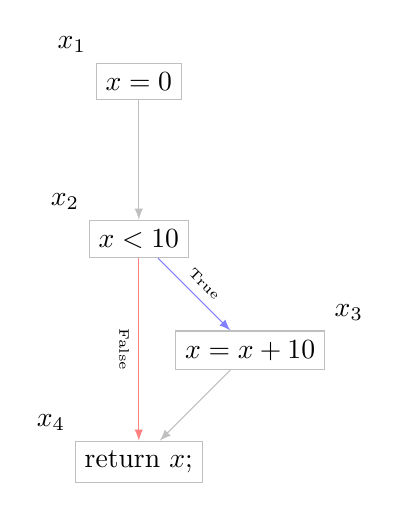
\begin{tikzpicture}
  [node distance=2cm, auto, 
  noline/.style={draw, -latex, draw=red!50, anchor=south, sloped}, 
  yesline/.style={draw, -latex, draw=blue!50, anchor=south, sloped}, 
  line/.style={draw, -latex, draw=black!25},
  block/.style={rectangle, draw=black!25}]
  % nodes
  \node [block] (init) {\(x = 0\)};
  \node [above left] at (init.north west) {\(x_1\)};
  \node [rectangle, draw=black!25, below of=init] (decide) {\(x < 10\)};
  \node [above left] at (decide.north west) {\(x_2\)};
  \node [rectangle, draw=black!25, below right of=decide] (then) {\(x = x + 10\)};
  \node [above right] at (then.north east) {\(x_3\)};
  \node [rectangle, draw=black!25, below left of=then] (end) {return \(x\);};
  \node [above left] at (end.north west) {\(x_4\)};

  % edges
  \path [line] (init) -- (decide);
  \path [yesline] (decide) -- node [above, font=\tiny] {True} (then);
  \path [line] (then) -- (end);
  \path [noline] (decide) --  node [below, font=\tiny] {False}  (end);

\end{tikzpicture}
\end{center}
\end{minipage}
\caption{}
\label{fig:codiceEsempio1}
\end{figure}

Supponiamo di usare come dominio semantico concreto l'insieme delle parti dei numeri interi che forma il reticolo \(\langle\wp(\mathbb{Z}), \cup, \cap, \emptyset, \mathbb{Z}\rangle\).
Il sistema di equazioni equivalente per trovare la collecting semantics è:
\[
F = 
\begin{cases}
   x_1 = \emptyset \\ 
   x_2 = \{0\} \\
   x_3 = \textrm{if}_{[x < 10]}(x_2) \\
   x_4 = \textrm{else}_{[x < 10]}(x_2) \cup (x_3 + \{10\}) \\
\end{cases}
\]

dove la funzione \(\textrm{if}_{[st]}:\wp(\mathbb{Z})\rightarrow\wp(\mathbb{Z})\) filtra i valori passati in input lasciando passare solo quelli che soddisfano la candizione in \(st\) (\(\textrm{else}_{[st]}:\wp(\mathbb{Z})\rightarrow\wp(\mathbb{Z})\) è simile ma fa passare solo quelli che non soddisfano la condizione \(st\)) e la funzione \(+:\wp(\mathbb{Z})\times\wp(\mathbb{Z})\rightarrow\wp(\mathbb{Z})\) somma elemento per elemento i valori dei due insiemi di interi passati come input. 

La collecting semantics sarà pari al least fix-point del sistema di equazioni \(F\) che è uguale al least upper bound tra tutti gli step della iterazione di Kleene (mostrata nel teorema [?]) di \(F\) su \(\wp(\mathbb{Z})^{|N|}\) partendo dal valore bottom di \(\wp(\mathbb{Z})\), ovvero \(\emptyset\), per ogni nodo.  

Per questo semplice esempio possiamo facilmente trovare il least fix-point. Partiamo da un vettore con tutti valori bottom:

\begin{figure}[H]
    \centering
\[
\arraycolsep=1.1pt
\begin{array}{ccccccccccc}
    \begin{tabular}{l}
    $
    t_0
    $ \\
    $
    \begin{bmatrix}
       \perp \\
       \perp \\
       \perp \\
       \perp
    \end{bmatrix}
    $
    \end{tabular}
    &
    \Longrightarrow
    &
    \begin{tabular}{l}
    $t_1$ \\
    $
    \begin{bmatrix}
       \perp \\
       \{0\} \\
       \perp \\
       \perp
    \end{bmatrix}
    $
    \end{tabular}
    &
    \Longrightarrow
    &
    \begin{tabular}{l}
    $t_2$ \\
    $
    \begin{bmatrix}
       \perp \\
       \{0\} \\
       \{0\} \\
       \perp
    \end{bmatrix}
    $
    \end{tabular}
    &
    \Longrightarrow
    &
    \begin{tabular}{l}
    $t_3$ \\
    $
    \begin{bmatrix}
       \perp \\
       \{0\} \\
       \{0\} \\
       \{10\}
    \end{bmatrix}
    $
    \end{tabular}
    &
    \Longrightarrow
    &
    \begin{tabular}{l}
    $t_4$ \\
    $
    \begin{bmatrix}
       \perp \\
       \{0\} \\
       \{0\} \\
       \{10\}
    \end{bmatrix}
    $
    \end{tabular}
    &
    \Longrightarrow
    &
    \cdots
\end{array}
\]
    \caption{Progressione della soluzione attraverso l'applicazione del sistema di equazioni \(F\)}
    \label{fig:progression}
\end{figure}

Ad ogni step applichiamo il sistema di equazioni \(F\). La serie è stazionaria dopo il quarto step. A questo punto facendo il lub di tutti gli step, ovvero \(\bigcup_{i\geq 0} t_i\), otteniamo il least fix-point che è uguale al terzo step e a tutti quelli dopo.
\end{example}

A questo punto una interpretazione astratta sarà a sua volta un sistema di equazioni:
\[F^{\natural} = \{x_i = f_i^{\natural}(x_1, x_2, \cdots, x_{|N|})\ |\ i=1, 2,\cdots, |N|\}\]
in cui sostituiamo le funzioni trasformatrici concrete con delle \textit{funzioni trasformatrici astratte} \(f_i^{\natural}:\mathbb{A}^{|N|}\rightarrow\mathbb{A}\) che approssimano correttamente quelle concrete e che ragionano su un dominio semantico astratto \(\mathbb{A}\) collegato tramite una connessione di Galois a quello concreto \(\mathbb{C}\). Per dimostrare la soundness dell'interpetazione astratta bisogna dimostrare la soundness di ogni funzione trasformatrice astratta in rispetto a quella concreta. 

Riprendendo l'esempio \ref{ex:easyCode} e sostituendo il dominio concreto con il dominio astrtatto degli intervalli di interi \(\langle\textrm{Int}, \preceq_{\textrm{Int}}, \sqcup, \sqcap, [-\infty, +\infty], \perp_{\textrm{Int}} \rangle\) il sistema di equazioni diventa: 

\[
F^{\natural} = 
\begin{cases}
   x_1 = \perp_{\textrm{Int}} \\ 
   x_2 = [0, 0] \\
   x_3 = \textrm{if}_{\textrm{Int}[x < 10]}(x_2) \\
   x_4 = \textrm{else}_{\textrm{Int}[x < 10]}(x_2) \sqcup (x_3 +_{\textrm{Int}} [10, 10]) \\
\end{cases}
\]
La sequenza di iterazioni di Kleene partendo da bottom di \(F^{\natural}\) diventa:

\begin{figure}[H]
    \centering
\[
\arraycolsep=1.1pt
\begin{array}{ccccccccccc}
    \begin{tabular}{l}
    $
    t_0
    $ \\
    $
    \begin{bmatrix}
       \perp_{\textrm{Int}} \\
       \perp_{\textrm{Int}} \\
       \perp_{\textrm{Int}} \\
       \perp_{\textrm{Int}}
    \end{bmatrix}
    $
    \end{tabular}
    &
    \Longrightarrow
    &
    \begin{tabular}{l}
    $t_1$ \\
    $
    \begin{bmatrix}
       \perp_{\textrm{Int}} \\
       [0, 0] \\
       \perp_{\textrm{Int}} \\
       \perp_{\textrm{Int}}
    \end{bmatrix}
    $
    \end{tabular}
    &
    \Longrightarrow
    &
    \begin{tabular}{l}
    $t_2$ \\
    $
    \begin{bmatrix}
       \perp_{\textrm{Int}} \\
       [0, 0] \\
       [0, 0] \\
       \perp_{\textrm{Int}}
    \end{bmatrix}
    $
    \end{tabular}
    &
    \Longrightarrow
    &
    \begin{tabular}{l}
    $t_3$ \\
    $
    \begin{bmatrix}
       \perp_{\textrm{Int}} \\
       [0, 0] \\
       [0, 0] \\
       [10, 10]
    \end{bmatrix}
    $
    \end{tabular}
    &
    \Longrightarrow
    &
    \begin{tabular}{l}
    $t_4$ \\
    $
    \begin{bmatrix}
       \perp_{\textrm{Int}} \\
       [0, 0] \\
       [0, 0] \\
       [10, 10]
    \end{bmatrix}
    $
    \end{tabular}
    &
    \Longrightarrow
    &
    \cdots
\end{array}
\]
    \caption{Progressione della soluzione attraverso l'applicazione del sistema di equazioni \(F^{\natural}\)}
    \label{fig:progression_abstr}
\end{figure}

Anche in questo caso dopo il terzo step la catena diventa stazionaria e facendo il lub di tutti gli step, quindi \(\bigsqcup_{i\geq0}t_i\), otteniamo il lfp di \(F^{\natural}\) che è pari a \(t_3\) ed a tutti gli step dopo.

In questo caso l'interpretazione astratta ci restituisce lo stesso risulato della analisi concreta in un tempo finito. Non saremo però sempre così fortunati, infatti anche nella computazione astratta possono formarsi catene crescenti infinite o troppo lunghe per essere calcolate in un tempo ragionevole. Abbiamo quindi bisogno di un estrapolatore in grado di far convergere il calcolo della approssimazione nel caso questa diverga o ci impieghi troppo tempo. Per questo motivo introduciamo gli operatori definiti nella sezione seguente.

\subsection{Widening e Narrowing}
Solo nel caso in cui il dominio astratto è finito o rispetta la condizione di catena crescente saremo sicuri che la computazione del fix-point finisce in un tempo finito. In tutti gli altri casi avremo bisogno di un operatore in grado di aiutarci a ristabilire la convergenza del calcolo.

\begin{definition}[Widening]
Dato un poset \(\simplePoset{S}\), la funzione \(\nabla:S\times S\rightarrow S\) è detta \textit{widening} se rispetta le seguenti condizioni:
\begin{itemize}
	\item per ogni coppia di elementi \(x, y\in S\) si ha che \(x\preceq_S x\nabla y\) e \(y\preceq_S x\nabla y\);
	\item per ogni catena crescente \(s_0\preceq_S s_1\preceq_S\cdots\preceq_S s_k\preceq_S\cdots\) la catena crescente: 
	\begin{align*}
	y_0 &= s_0\\
	y_{n+1} &= y_n\nabla x_{n+1}
	\end{align*}
	è stazionaria, ovvero \(\exists k\ge 0:\forall t\geq k: y_t = y_k\)
\end{itemize}
\end{definition}
Il widening è quindi una over-approsimazione del lub. 

\begin{definition}[Iterazione ascendente con widening]
Dati un poset \(\simplePoset{S}\), una funzione \(f:S\rightarrow S\) ed un widening \(\nabla : S\times S\rightarrow S\), la sequenza di iterazione con \(\nabla\) su \textit{S}, partendo dall'elemento \(\perp\in S\) è definito ricorsivamente nel seguente modo, \(\forall \ n \in \mathbb{N}\):
\begin{align*}
x_0 &= \perp \\
x_{n+1} &=  \begin{cases}
            x_n &\textrm{se} f(x_n)\preceq_S x_n \\
            x_n \nabla f(x_n) &\textrm{altrimenti}
            \end{cases}
\end{align*}
Ogni sequenza di iterazioni di \textit{f}, avente un widening \(\nabla\), è stazionaria dopo un numero finito di step ed il suo limite, \(x^{\nabla}\), è un post-fixpoint di \textit{f} e vale \(\textrm{lfp}(f)\preceq x^{\nabla}\). 
\end{definition}

Questo ultimo risultato ci dice che applicando il widening otterremo in un tempo finito una approssimazione sound del least fix-point di \(f\). Quello che in pratica si fa non è applicare il widening ad ogni step (anche se possibile) ma applicarlo solo in certi selezionati passaggi per mitigare gli effetti di over-approssimazione che comporta mantenendo la sua capacità di far convergere la computazione. Un altro modo che abbiamo di attenuare l'effetto di approssimazione del widening è quello di far seguire la fase ascendente della computazione con una fase discendente, in cui al posto del lub verrà utilizzato il glb e al posto del widening si userà un altro operatore, il narrowing.

Più generalmente se abbiamo un reticolo completo \(\completeLattice{S}\), partendo da un post-fix-point \(s\in S\) di una funzione continua \(f:S\rightarrow S\) si può scendere verso il più grande fix-point minore od uguale ad \(s\) facendo il glb di tutti gli elementi della catena discendente formata dalla iterazione di Kleene di \(f\) partendo da \(s\), ovvero \(\textrm{gfp}_s(f)=\bigsqcap\{f^n(s)\ |\ n\geq 0\}\). 

Una idea è quella di usare come post-fix-point da cui iniziare la computazione discendente il risultato della fase ascendente, calcolata con il widening, di cui abbiamo dimostrato che il limite è post-fix-point della funzione.

Come nella fase ascendente, anche discendendo il dominio si può incappare in catene infinite se il reticolo non rispetta la condizione di catena discendente. Per questo motivo abbiamo bisogno di un operatore di interpolazione che accelleri o forzi la convergenza della iterazione di sequenze decrescenti. Questo operatore lo chiamiamo narrowing e lo definiamo così:

\begin{definition}[Narrowing]
Dato un poset \(\simplePoset{S}\), la funzione \(\Delta:S\times S\rightarrow S\) è detta \textit{narrowing} se rispetta le seguenti condizioni:
\begin{itemize}
	\item per ogni coppia di elementi \(x, y\in S\) se \(x\preceq_S y\) si ha che \(x\preceq_S (x\Delta y) \preceq_S y\);
	\item per ogni catena decrescente \(s_0\succeq_S s_1\succeq_S\cdots\succeq_S s_k\succeq_S\cdots\) la catena decrescente: 
	\begin{align*}
	y_0 &= s_0\\
	y_{n+1} &= y_n\nabla x_{n+1}
	\end{align*}
	è stazionaria, ovvero \(\exists k\ge 0:\forall t\geq k: y_t = y_k\)
\end{itemize}
\end{definition}

\begin{definition}[Iterazione discendente con narrowing]
Dati un poset \(\simplePoset{S}\), una funzione Scott-continua \(f:S\rightarrow S\), un narrowing \(\Delta : S\times S\rightarrow S\), la sequenza di iterazione con \(\Delta\) su \textit{S}, partendo da un post-fix-point \(x^{\nabla}\in S\) di \(f\) è definito ricorsivamente nel seguente modo, \(\forall \ n \in \mathbb{N}\):
\begin{align*}
y_0 &= x^{\nabla} \\
y_{n+1} &=  \begin{cases}
            y_n &\textrm{se} f(y_n) = y_n \\
            y_n \Delta f(y_n) &\textrm{altrimenti}
            \end{cases}
\end{align*}
Questa sequenza decrescente è stazionaria dopo un numero finito di passaggi ed in più il suo limite \(y^{\Delta}\) è un post-fix-point di \(f\) ed è una approssimazione del least-fix-point di \(f\) e vale che:
\[\textrm{lfp}(f)\preceq_S y^{\Delta}\preceq_S x^{\nabla}\]
\end{definition}



\begin{example}
Per il dominio degli intervalli interi possiamo definire un widening \(\nabla:\textrm{Int}\times\textrm{Int}\rightarrow\textrm{Int}\) in questo modo: 
\[\forall x\in \textrm{Int}: \perp\nabla x = x\nabla\perp = x \textrm{ e } \]
\[
[l_0, u_0]\nabla[l_1, u_1] = 
\begin{cases}
    [l_0, u_0] & \textrm{se } l_0\leq l_1 \wedge u_0 \geq u_1 \\
    [-\infty, u_0] & \textrm{se } l_1 < l_0 \wedge u_0 \geq u_1 \\
    [l_0, +\infty] & \textrm{se } l_0\leq l_1 \wedge u_1 > u_0 \\
    [-\infty, +\infty] & \textrm{se } l_1 < l_0 \wedge u_1 > u_0 \\
\end{cases}
\]

ed un narrowing \(\Delta:\textrm{Int}\times\textrm{Int}\rightarrow\textrm{Int}\) in questo modo: 
\[\forall x\in \textrm{Int}: \perp\nabla x = x\nabla\perp = \perp \textrm{ e } \]
\[
[l_0, u_0]\nabla[l_1, u_1] = 
\begin{cases}
    [l_1, u_1] & \textrm{se } l_0 = -\infty \wedge u_0 = +\infty \\
    [l_0, u_1] & \textrm{se } l_0 \neq -\infty \wedge u_0 = +\infty \\
    [l_1, u_0] & \textrm{se } l_0 = -\infty \wedge u_0 \neq +\infty \\
    [l_0, u_0] & \textrm{se } l_0 \neq -\infty \wedge u_0 \neq +\infty \\
\end{cases}
\]
\end{example}

Riassumendo il concetto nella prima fase (ascendente) utilizzeremo, per raggiungere un post-fix-point di \(F^{\natural}\), una versione del sistema di equazione che fa il join tra gli step della iterazione utilizzando il lub od il widening (con una logica in grado di decidere quando usare l'uno o l'altro), questo passaggio lo chiamiamo \(F^{\nabla}\). Nella fase discendente invece, partendo dal risultato calcolato da quella prima, modificheremo il sistema di equazioni in modo da fare il meet tra gli step utlizzando o il glb o il narrowing, questo passaggio lo chiamiamo \(F^{\Delta}\). 
In figura \ref{fig:phasesFig} è mostrata una rappresentazione grafica del della fase ascendente e discendente su un dominio \(\mathbb{S}\).

\begin{figure}[H]
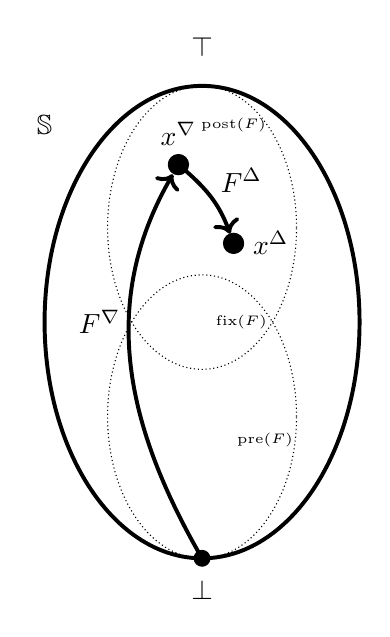
\begin{tikzpicture}
    \draw [line width=0.5mm] (0, 0) ellipse (2cm and 3cm);
    \node (top) at (0, 3.5) {$\top$};
    \node (bottom) at (0, -3.4) {$\perp$};
    \draw [densely dotted] (0, -1.2) ellipse (1.2cm and 1.8cm);
    \draw [densely dotted] (0, 1.2) ellipse (1.2cm and 1.8cm);
    \node (bottomStart) at (0, -3) {};
    \node (domain) at (-2, 2.5) {\(\mathbb{S}\)};
    \node (pre) at (0.8, -1.5)  {\tiny pre($F$)};
    \node (post) at (0.4, 2.5)  {\tiny post($F$)};
    \node (fix) at (0.5, 0)  {\tiny fix($F$)};
    \node [label=above:{$x^{\nabla}$}] (widPost) at (-0.3, 2) {};
    \draw [fill=black] (0, -3) circle (0.1cm);

    \node (fnabla) at (-1.3, 0) {\(F^{\nabla}\)};
    \node (fDelta) at (0.5, 1.8) {\(F^{\Delta}\)};
    
    \node [label=right:{$x^{\Delta}$}] (narrPost) at (0.4, 1) {};
    \draw [fill=black, line width=0.1mm] (0.4, 1) circle (0.13cm);
    
    \draw [fill=black, line width=0.1mm] (-0.3, 2) circle (0.13cm);

    \draw[->, line width=0.5mm] (bottomStart.center) to [out=120, in=240] (widPost);

    \draw[->, line width=0.5mm] (widPost.center) to [out=320, in=110] (narrPost);
\end{tikzpicture}
    \centering
    \caption{Fase ascendente e discendente su un dominio \(\mathbb{S}\)}
    \label{fig:phasesFig}
\end{figure}

\begin{figure}
\begin{minipage}{1cm}
\hspace{1cm}
\end{minipage}
\begin{minipage}[c][5cm][c]{0.5\textwidth-2cm}
\vspace{\fill}
\begin{lstlisting}[language=Python, numbers=none]
x = 0
if x < 100:
    if x < 50:
        x = x + 2;
    else
        x = x +10;
return x;
\end{lstlisting}
\vspace{\fill}
\end{minipage}
\begin{minipage}{0.5\textwidth}
\begin{center}
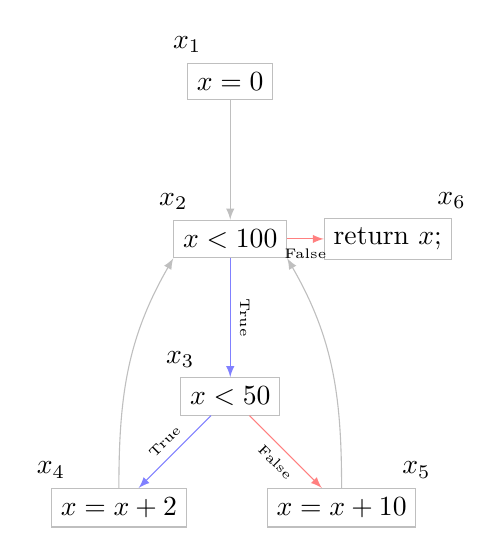
\begin{tikzpicture}
  [node distance=2cm, 
  noline/.style={draw, -latex, draw=red!50, anchor=south, sloped}, 
  yesline/.style={draw, -latex, draw=blue!50, anchor=south, sloped}, 
  line/.style={draw, -latex, draw=black!25},
  block/.style={rectangle, draw=black!25}]
  % nodes
  \node [block] (init) {\(x = 0\)};
  \node [above] at (init.north west) {\(x_1\)};
  \node [rectangle, draw=black!25, below of=init] (decide1) {\(x < 100\)};
  \node [above] at (decide1.north west) {\(x_2\)};
  \node [rectangle, draw=black!25, below of=decide1] (decide2) {\(x < 50\)};
  \node [above] at (decide2.north west) {\(x_3\)};
  \node [rectangle, draw=black!25, below left of=decide2] (then1) {\(x = x + 2\)};
  \node [above] at (then1.north west) {\(x_4\)};
  \node [rectangle, draw=black!25, below right of=decide2] (then2) {\(x = x + 10\)};
  \node [above] at (then2.north east) {\(x_5\)};
  \node [rectangle, draw=black!25, right of=decide1] (return) {return \(x\);};
  \node [above] at (return.north east) {\(x_6\)};
  % edges
  \path [line] (init) -- (decide1);
  \path [yesline] (decide1) -- node [above, font=\tiny] {True} (decide2);
  \path [noline] (decide1) --  node [below, font=\tiny] {False}  (return);
  \path [yesline] (decide2) -- node [above, font=\tiny] {True} (then1);
  \path [noline] (decide2) --  node [below, font=\tiny] {False}  (then2);
  \path [line] (then1)  [out=90, in=240] to (decide1.south west);
  \path [line] (then2.north)  [out=90, in=300] to (decide1.south east);
\end{tikzpicture}
\end{center}
\end{minipage}
\caption{}
\label{fig:codiceEsempio2}
\end{figure}

\begin{example}\label{ex:esempio2}
Nell'esempio che mostreremo ora analizzeremo il codice in \ref{fig:codiceEsempio2} cerrcando una approssimazione della collecting semantics tramite interpretazione astratta usando il dominio degli intervalli interi. Nella figura \ref{fig:ris} è mostrata anche il sistema di equazioni astratte di cui cerchiamo la soluzione minima. A differenza dell'esempio \ref{ex:easyCode} risoleveremo il sistema di equazioni in modo diverso, infatti adesso calcoleremo entrambe le fasi (ascendente e discendente) ed utilizzeremo gli operatori di widening e narrowing per velocizzare la convergenza del calcolo, in questo modo: 
\[
F^{\nabla} = 
\begin{cases}
    x_i = x_i \nabla f_i(x_1, x_2, \cdots, x_n) & \textrm{se il nodo \textit{i} è un WP} \\
    x_i = x_i \sqcup f_i(x_1, x_2, \cdots, x_n) & \textrm{altrimenti} \\
\end{cases}
\]
per la fase ascendente, e:
\[
F^{\Delta} = 
\begin{cases}
    x_i = x_i \Delta f_i(x_1, x_2, \cdots, x_n) & \textrm{se il nodo \textit{i} è un WP} \\
    x_i = x_i \sqcap f_i(x_1, x_2, \cdots, x_n) & \textrm{altrimenti} \\
\end{cases}
\]
per la fase discendente.

Per WP intendiamo i \textit{widening points}, ovvero i punti del CFG in cui viene applicato il widening. Si può mostrare che per ogni ciclo del grafo si può etichettare un nodo al suo interno come WP e il calcolo del fix-point convergerà comunque (questo ci permette di essere più selettivi nell'uso del widening e quindi migliorare la precisione dell'approssimazione). Per questo esempio abbiamo \(x_3\) come unico WP.

I risultati dell'analisi sono mostrati nella tabelle della figura \ref{fig:ris}.
\begin{figure}[H]
\begin{minipage}{\textwidth}
\vspace{1cm}
\[
F^{\natural}=
\begin{cases}
    x_1 = \top \\
    x_2 = [0, 0]\sqcup(x_4 +_{\textrm{Int}} [2, 2])\sqcup(x_5 +_{\textrm{Int}} [10, 10]) \\
    x_3 = \textrm{if}_{[x<100]}(x_2) \\
    x_4 = \textrm{if}_{[x<50]}(x_3) \\
    x_5 = \textrm{else}_{[x<50]}(x_3) \\
    x_6 = \textrm{else}_{[x<100]}(x_2) \\
\end{cases}
\]  
\centering
(a)
\end{minipage}
\begin{minipage}{\textwidth}
    \centering
    \vspace{1cm}
        \[
        \begin{tabular}{|c|c|c|c|c||c|c|c||}
        \hline
        \multicolumn{2}{|c|}{fase} & 
        \multicolumn{3}{c||}{\textbf{ascendente}} & 
        \multicolumn{2}{c|}{\textbf{discendente}}\\
        
        \hline 
        N & WP & 1st & 2nd & 3rd=$x^{\nabla}$ & 1st & 2nd=$x^{\Delta}$  \\
        \hline
        $x_1$ &  &  
            $\top$ & $\top$ & $\top$ & 
            $\top$ & $\top$ \\
        \hline
        $x_2$ &  & 
            $\left[0, 0\right]$ & $\left[0, 2\right]$ & $\left[0, +\infty \right]$ & 
            $\left[0, +\infty \right]$ & $\left[0, 109\right]$ \\
        \hline
        $x_3$ & \checkmark & 
            $\left[0, 0\right]$ & $\left[0, +\infty \right]$ & $\left[0, +\infty \right]$ & 
            $\left[0, 99\right]$ & $\left[0, 99\right]$ \\
        \hline
        $x_4$ &  & 
            $\left[0, 0\right]$ & $\left[0, 49\right]$ & $\left[0, 49\right]$ & 
            $\left[0, 49\right]$ & $\left[0, 49\right]$ \\
        \hline
        $x_5$ &  & 
            $\perp$ & $\left[50, +\infty \right]$ & $\left[50, +\infty \right]$ & 
            $\left[50, 99\right]$ & $\left[50, 99\right]$ \\
        \hline
        $x_6$ &  & 
            $\perp$ & $\left[100, +\infty \right]$ & $\left[100, +\infty \right]$ & 
            $\left[100, +\infty \right]$ & $\left[100, 109\right]$ \\
        \hline
        \end{tabular}
        \]
        (b)
    \end{minipage}
    \caption{(a) sistema di equazioni astratte per il CFG in \ref{fig:codiceEsempio2} (b) tabella dei risultati divisi per step e fase.}
    \label{fig:ris}
\end{figure}
\end{example}
\chapter{Decoupling della fase ascendente e fase discendente}\label{chapter:decoupling}

Nel capitolo precedente abbiamo visto come si può usare l'interpretazione astratta per l'analisi statica di un programma. Il metodo proposto si compone di una astrazione del dominio concreto, quindi una connessione di Galois \(\mathbb{C}\galois{\alpha}{\gamma}\mathbb{A}\),  ed un sistema di equazioni  astratte \(F_{\mathbb{A}}\) che correttamente approssimano il comportamento del programma. Il calcolo avviene poi in due fasi, una prima fase, detta ascendente, che calcola un post-fix-point di \(F_{\mathbb{A}}\) in cui si utilizza un estrapolatore (come il widening) per assicurare la convergenza seguita da una fase discendente che ne migliora i risultati. Va notato che entrambi le fasi vengono eseguite sullo stesso dominio \(\mathbb{A}\).

L'idea proposta in [??] è quella di disaccoppiare (decouple) le due fasi, ovvero di calcolare la fase discendente su un dominio diverso, e più preciso, rispetto a quello della fase ascendente. L'obbiettivo è quello di ottenere una analisi più precisa senza pagare il costo in termini di efficienza del calcolare la fase ascendente con un dominio molto preciso. In più la fase discendente può essere stoppata dopo un qualsiasi numero di iterazioni e comunque fornire un risultato corretto. Per questo può essere più facile ottenere un buon tradeoff tra precisione ed efficienza.

La notazione che verrà usata per indicare questo approccio decoupled all'interpretazione astratta è \(\mathbb{A}\uparrow\downarrow\mathbb{D}\), dove \(\mathbb{A}\) è il dominio astratta usato nella fase ascendente e \(\mathbb{D}\) è quello utilizzato nella fase discendente. Con questo metodo avremo bisogno di una doppia connessione di Galois in questo modo \(\mathbb{C}\galois{\alpha_{\mathbb{A}}}{\gamma_{\mathbb{D}}}\mathbb{D}\galois{\alpha_{\mathbb{D}\uparrow\downarrow\mathbb{D}}}{\gamma_{\mathbb{A}\uparrow\downarrow\mathbb{D}}}\mathbb{A}\) ed è richiesto che la funzione di concretizzazione \(\gamma_{\mathbb{A}\uparrow\downarrow\mathbb{D}}\) sia calcolabile. L'approccio decoupled è graficamente rappresentato nella figura \ref{fig:decFig}. Avendo un sistema di equazioni concrete \(F_{\mathbb{C}}\) correttamente approssimato dal sistema di equazioni \(F_{\mathbb{D}}\) sul dominio \(\mathbb{D}\), e queste ultime ulteriormente approssimate da \(F_{\mathbb{A}}\) sul dominio \(\mathbb{A}\), possiamo riassumere i passaggi del metodo decoupled in questo modo: (1) nella fase ascendente calcoliamo il post-fixpoint \(x^{\nabla}_{\mathbb{A}}\in\mathbb{A}\) di \(F^{\nabla}_{\mathbb{A}}\) con il widening, (2) poi trasferiamo \(x^{\nabla}_{\mathbb{A}}\) nel dominio più preciso \(\mathbb{D}\) tramite la funzione concretizzante \(\gamma_{\mathbb{A}\uparrow\downarrow\mathbb{D}}\), (3) ed infine nella fase discendente si calcola un post-fix-point migliorato \(x^{\Delta}_{\mathbb{D}}\in\mathbb{D}\) usando il sistema di equazioni \(F^{\Delta}_{\mathbb{D}}\) con narrowing partendo da  \(\gamma_{\mathbb{A}\uparrow\downarrow\mathbb{D}}(x^{\nabla}_{\mathbb{A}})\).

\begin{figure}[H]
\centering
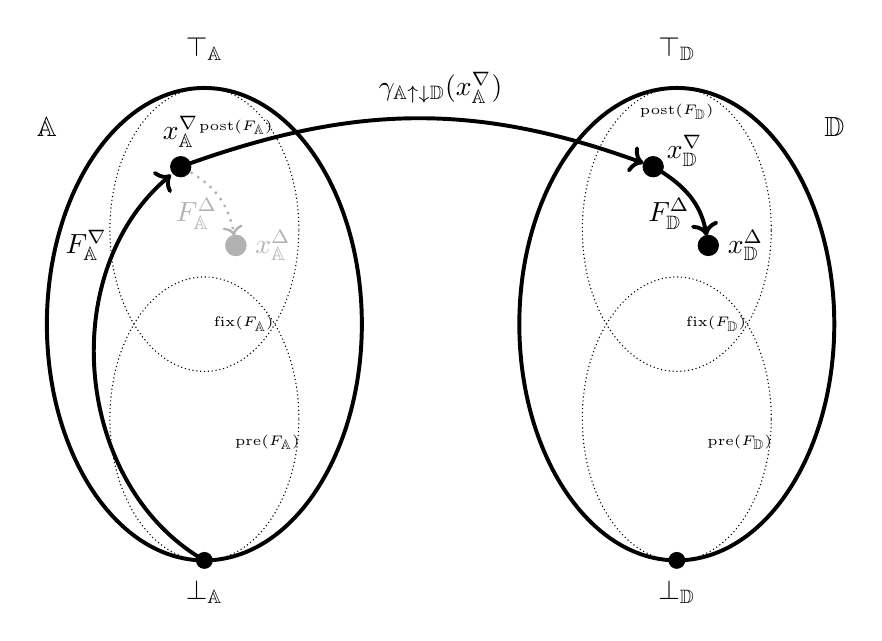
\begin{tikzpicture}
    \draw [line width=0.5mm] (-3, 0) ellipse (2cm and 3cm);
    \draw [line width=0.5mm] (3, 0) ellipse (2cm and 3cm);
    
    \node (top) at (-3, 3.5) {$\top_{\mathbb{A}}$};
    \node (bottom) at (-3, -3.4) {$\perp_{\mathbb{A}}$};
    \node (top) at (3, 3.5) {$\top_{\mathbb{D}}$};
    \node (bottom) at (3, -3.4) {$\perp_{\mathbb{D}}$};
    
    \draw [densely dotted] (-3, -1.2) ellipse (1.2cm and 1.8cm);
    \draw [densely dotted] (-3, 1.2) ellipse (1.2cm and 1.8cm);
    \draw [densely dotted] (3, -1.2) ellipse (1.2cm and 1.8cm);
    \draw [densely dotted] (3, 1.2) ellipse (1.2cm and 1.8cm);
    
    \node (domain) at (-5, 2.5) {\(\mathbb{A}\)};
    \node (domain) at (5, 2.5) {\(\mathbb{D}\)};
    
    \node (bottomStartA) at (-3, -3) {};
    \draw [fill=black] (-3, -3) circle (0.1cm);
    \node (bottomStartD) at (3, -3) {};
    \draw [fill=black] (3, -3) circle (0.1cm);

    \node (pre) at (-2.2, -1.5)  {\tiny pre($F_{\mathbb{A}}$)};
    \node (post) at (-2.6, 2.5)  {\tiny post($F_{\mathbb{A}}$)};
    \node (fix) at (-2.5, 0)  {\tiny fix($F_{\mathbb{A}}$)};
    \node (pre) at (3.8, -1.5)  {\tiny pre($F_{\mathbb{D}}$)};
    \node (post) at (3, 2.7)  {\tiny post($F_{\mathbb{D}}$)};
    \node (fix) at (3.5, 0)  {\tiny fix($F_{\mathbb{D}}$)};
    
    \node [label=above:{$x^{\nabla}_{\mathbb{A}}$}] (widPostA) at (-3.3, 2) {};
    \draw [fill=black, line width=0.1mm] (-3.3, 2) circle (0.13cm);
    \node (widPostD) at (2.7, 2) {};
    \node (widPostDlabel) at (3.1, 2.2) {$x^{\nabla}_{\mathbb{D}}$};
    \draw [fill=black, line width=0.1mm] (2.7, 2) circle (0.13cm);

    \node (fnablaA) at (-4.5, 1) {\(F^{\nabla}_{\mathbb{A}}\)};
    \node (fDeltaA) at (-3.1, 1.4) {\color{black!30}\(F^{\Delta}_{\mathbb{A}}\)};
    \node (fDeltaD) at (2.9, 1.4) {\(F^{\Delta}_{\mathbb{D}}\)};

    \node (concret) at (0, 3) {\(\gamma_{\mathbb{A}\uparrow\downarrow\mathbb{D}}(x^{\nabla}_{\mathbb{A}})\)};
    
    \node [label=right:{\color{black!30}$x^{\Delta}_{\mathbb{A}}$}] (narrPostA) at (-2.6, 1) {};
    \draw [black!30, fill=black!30] (-2.6, 1) circle (0.13cm);
    \node [label=right:{$x^{\Delta}_{\mathbb{D}}$}] (narrPostD) at (3.4, 1) {};
    \draw [fill=black, line width=0.1mm] (3.4, 1) circle (0.13cm);

    \draw[->, line width=0.5mm] (bottomStartA.center) to [out=150, in=220] (widPostA);

    \draw[->, line width=0.3mm, dotted, black!30] (widPostA) to [out=330, in=100] (narrPostA);
    
    \draw[->, line width=0.5mm] (widPostD.center) to [out=330, in=100] (narrPostD);
    \draw[->, line width=0.5mm] (widPostA.center) to [out=20, in=160] (widPostD);
\end{tikzpicture}
    \centering
    \caption{Fase ascendente e discendente disaccoppiate sui domini \(\mathbb{A}\) e \(\mathbb{D}\))}
    \label{fig:decFig}
\end{figure}

\begin{example}
Riprendiamo l'esempio \ref{ex:esempio2} e utilizziamo il dominio decoupled \(\textrm{Sign}\uparrow\downarrow\textrm{Int}\) per cercare una approssimazione della collecting semantics del programma. La funzione concretizzante \(\gamma_{\textrm{Sign}\uparrow\downarrow\textrm{Int}}\) la abbiamo definita nell'esempio \ref{ex:galoisSignInt}. I risultati dell'analisi sono mostrati nella tabella in figura \ref{fig:risDecSingInt}. 

\begin{figure}[H]
\begin{minipage}{\textwidth}
    \centering
    \vspace{1cm}
        \[
        \begin{tabular}{|c|c|c|c||c||c|c|c||}
        \hline
        \multicolumn{2}{|c|}{fase} & 
        \multicolumn{2}{c||}{\textbf{ascendente}} & 
        \multicolumn{1}{c||}{\textbf{decoupling}} & 
        \multicolumn{2}{c|}{\textbf{discendente}}\\
        
        \hline 
        \rule{0pt}{14pt} N & WP & 1st & 2nd=\(x^{\nabla}_{\textrm{Sign}}\) & 
        \(\gamma_{\textrm{Sign}\uparrow\downarrow\textrm{Int}}(x^{\nabla}_{\textrm{Sign}})\)& 
        1st & 2nd=\(x^{\Delta}_{\textrm{Int}}\)  \\
        \hline
        $x_1$ &  &  
            $\top_{\textrm{Sign}}$ & $\top_{\textrm{Sign}}$ & 
            $\top_{\textrm{Int}}$ & 
            $\top_{\textrm{Int}}$ & $\top_{\textrm{Int}}$ \\
        \hline
        $x_2$ &  & 
            0 & 0+ & 
            $\left[0, +\infty \right]$ & 
            $\left[0, +\infty \right]$ & $\left[0, 109\right]$ \\
        \hline
        $x_3$ & \checkmark & 
            0 & 0+ & 
            $\left[0, +\infty \right]$ & 
            $\left[0, 99\right]$ & $\left[0, 99\right]$ \\
        \hline
        $x_4$ &  & 
            0 & 0+ & 
            $\left[0, +\infty\right]$ & 
            $\left[0, 49\right]$ & $\left[0, 49\right]$ \\
        \hline
        $x_5$ &  & 
            $\perp_{\textrm{Sign}}$ & + & 
            $\left[1, +\infty \right]$ & 
            $\left[50, 99\right]$ & $\left[50, 99\right]$ \\
        \hline
        $x_6$ &  & 
            $\perp_{\textrm{Sign}}$ & + & 
            $\left[1, +\infty \right]$ & 
            $\left[100, +\infty \right]$ & $\left[100, 109\right]$ \\
        \hline
        \end{tabular}
        \]
    \end{minipage}
    \caption{tabella dei risultati del dominio \(\textrm{Sign}\uparrow\downarrow\textrm{Int}\) divisi per step e fase.}
    \label{fig:risDecSingInt}
\end{figure}
\end{example}

%\chapter{Progettazione}\label{chapter:progettazione}
\Blindtext
%\chapter{Risultati}\label{chapter:res}
\Blindtext %Dummy Text - remove
%
%
%%%% Le Conclusioni
\pagestyle{plain}
\chapter*{Conclusione} %Se si cambia il Titolo cambiare anche la riga successiva così che appia corretto nell'conclusione
\addcontentsline{toc}{chapter}{Conclusione} %Per far apparire Introduzione nell'indice (Il nome deve rispecchiare quello del chapter)
Conclusione che riassume il lavoro svolto ed eventuali lavori futuri.

\blindtext %Dummy Text - remove
\blindtext %Dummy Text - remove
%
%%%% La bibliografia
\bibliographystyle{apalike} %{plain} -- Scegliere lo stile preferito
\bibliography{./Bibliografia}
%
\chapter*{Ringraziamenti}

%
% Le appendici
\appendix
\chapter{Appendice di Esempio}
\Blindtext
%
\end{document}